\chapter{Reconstrucción e Identificación de objetos físicos} \label{chap:ch3}

\newthought{En este capítulo} describiremos la reconstrucción e identificación de objetos físicos, candidatos a electrones, muones, jets hadrónicos y taus, a partir de las señales de los detectores de ATLAS. En particular, para el caso de pares de $\tau$ con reducida separación angular $\Delta R < 1$ --que son de interés para este trabajo--, donde los métodos tradicionales fallan, introduciremos un novedoso método que hará posible su uso en el canal de decaimiento hadrónico.

\section{Objetos de bajo nivel}

El proceso de reconstrucción e identificación offline de objetos en ATLAS se puede dividir globalmente en dos etapas: objetos de bajo nivel --como trazas (\textit{tracks}) y depósitos de energía en los calorímetros-- y objetos de alto nivel --como los electrones, muones, etc.--. En esta primera sección desarrollaremos la reconstrucción de los primeros, a partir de la información de alta granularidad proveniente del ID, MS y los calorímetros.

\subsection{Reconstrucción de Trazas}

En cada evento, las trazas son reconstruidas a partir de \textit{hits} en el ID, agrupándolos geométricamente en cada capa del Detector de Píxeles y el SCT. Tres de esos clusters son utilizados para conformar una semilla para la reconstrucción de un \textit{track}~\cite{Cornelissen2008a,Cornelissen2008,TheATLASCollaboration2017}.

Sin embargo, no siempre las semillas se corresponden a trazas físicas: puede ocurrir que una semilla de \textit{tracks} sea originada por una combinación no-física de \textit{hits} en los subsistemas del ID, es decir, por una mera coincidencia. Para reducir la incidencia de estos fenómenos exclusivamente combinatorios, se aplican cortes en el parámetro de impacto y el $p_T$ correspondiente a las semillas: $p_T > \SI{400}{\MeV}$, $\abs{\eta} < 2.5$, $\abs{d_0^{BL}} < \SI{2}{\milli\meter}$ y $\abs{z_0^{BL} \sin\theta} < \SI{3}{\milli\meter}$. Los parámetros de impacto transversales y longitudinales ($d_0^{BL}$ y $z_0^{BL}$ respectivamente) se definen en este caso respecto a los puntos de máxima aproximación al BL (\textit{beam line}, eje principal de ATLAS), de acuerdo a la \cref{fig:ch3:tracks_impact-param}. Su estimación se realiza suponiendo una trayectoria helicoidal de una partícula cargada en un campo magnético uniforme, corrigiendo las pérdidas de energía en el material. Además, la semilla deberá contener al menos 7 clusters del Detector de Píxeles y SCT (se esperan 12), y como máximo compartir un cluster en la misma capa del Detector de Píxeles con otro \textit{track}, o dos clusters en el SCT.


\begin{marginfigure}
    \centering
    \subfloat[][\label{fig:ch3:tracks_impact-param:d0}]{\resizebox{0.98\linewidth}{!}{
\begin{tikzpicture}[font=\large]
    \begin{axis}[
        scale only axis=true,
        width=50mm,
        height=47.5mm,
        xmin=-0.2, xmax=0.7, 
        ymin=-0.17, ymax=0.9,
        axis lines=middle,
        axis line style={-{Latex[round, scale=1.2]}, thick},
        ticks=none,
        clip=false,
    ]
    \addplot+[-{To[scale=1]}, mark=none, Burgundy, thick, domain=-0.14:0.63, smooth, samples=100] {1.3*((1-(x-0.77)^2)^(1/2) - 0.36)};
    \addplot[darkgray, dashed, thick, domain=-0.18:0.18, smooth, samples=100] {0.0709907 + 2.8533 * (0.14 + x)};
    %
    \draw[dotted, densely dotted, thick] (axis cs:0, 0) -- (axis cs:-0.14, 0.0709907) node[pos=0.4, above=0.05mm] {$d_0$};
    %
    \node at (axis cs:0.76, 0) {$x$};
    \node at (axis cs:0, 0.98) {$y$};
    \end{axis}
\end{tikzpicture}
}
}\\
    \subfloat[][\label{fig:ch3:tracks_impact-param:z0}]{\resizebox{0.98\linewidth}{!}{
\begin{tikzpicture}[font=\large]
    \begin{axis}[
        scale only axis=true,
        width=50mm,
        height=47.5mm,
        xmin=-0.2, xmax=0.7, 
        ymin=-0.17, ymax=0.9,
        axis lines=middle,
        axis line style={-{Latex[round, scale=1.2]}, thick},
        ticks=none,
        clip=false,
    ]
    \addplot+[-{To[scale=1]}, mark=none, Burgundy, thick, domain=0.1:0.63, smooth, samples=100] {-0.1 + 1.5 * (x - 0.1)};
    \draw[darkgray, dashed, thick] (axis cs:0.1, -0.15) -- (axis cs:0.1, 0.92);
    %
    \draw[dotted, densely dotted, thick] (axis cs:0, 0.4) -- (axis cs:0.1, 0.4) node[pos=0.5, above=0.05mm] {$z_0$};
    %
    \node at (axis cs:0.76, 0) {$z$};
    \node at (axis cs:0,0.98) {$r$};
    \end{axis}
\end{tikzpicture}
}
}

    \caption{Parámetros de impacto transversal $d_0$ \subref{fig:ch3:tracks_impact-param:d0} y longitudinal $z_0$ \subref{fig:ch3:tracks_impact-param:z0}. Cuando se utiliza el supraíndice ``$BL$'', estos se encuentran definidos respecto al punto de máxima aproximación al vértice primario, sobre la línea del haz de partículas.}
    \label{fig:ch3:tracks_impact-param}
\end{marginfigure}

Las trayectorias de las semillas que satisfacen los cortes de calidad son luego extrapoladas hasta el TRT utilizando un filtro de Kalman~\cite{Fruhwirth1987}, resultando en un \textit{candidato de track}. Cada candidato es posteriormente evaluado, asignando en una primera etapa una puntuación a partir de la calidad de los ajustes y extrapolaciones, y penalizando los \textit{hits} esperados pero faltantes en los distintos detectores. Esta puntuación, junto a un algoritmo de Redes Neuronales, son utilizados para resolver casos donde múltiples candidatos de trazas compartan señales en algunos de los detectores.

El conjunto resultante de candidatos de trazas es ajustado con el \textit{ATLAS global track fitter}, formando el conjunto final de trazas del evento. La carga y el momento asignado a cada \textit{track} son calculados a partir de la curvatura de las trayectorias ajustadas, en presencia del fuerte campo magnético producido por el solenoide central.


\subsection{Reconstrucción del Vértice Primario}

Debido al elevado número medio de interacciones simultáneas en cada \textit{bunch crossing}, como hemos notado en la \cref{sec:ch2:atlas:trigger}, es común que en cada evento capturado se hayan detectado partículas provenientes de más de una colisión pp. La reconstrucción de los vértices primarios --los puntos en el espacio donde ocurrió una colisión inelástica pp-- es, por lo tanto, fundamental para clasificar los objetos físicos reconstruidos.

El proceso de reconstrucción se realiza en dos etapas~\cite{Meloni2016,Boutle2017,ATL-PHYS-PUB-2015-026}. En un primer paso, las semillas de vértices se ubican en el plano transverso al punto de colisión del haz. La posición longitudinal es obtenida a partir de la distribución de las trazas reconstruidas, extrapoladas al punto de la colisión. En un segundo paso, se aplica un algoritmo de ajuste iterativo, donde en cada iteración las trazas menos compatibles con una semilla de vértice propuesta son descartados; el proceso finaliza con la convergencia del ajuste. Este procedimiento es repetido para cada semilla de vértice, eliminando las trazas ajustadas en las semillas anteriores. Finalmente, se elige como vértice primario de la interacción a aquel con el mayor valor del parámetro $\sum p_T^2$.


\subsection{Identificación de clusters en el Calorímetro}

Como hemos introducido en la \cref{sec:ch2:atlas:calo}, al alcanzar los calorímetros e interactuar con sus elementos pasivos\sidenote{$\textrm{LAr}$ en el caso del ECAL; principalmente $\textrm{Pb}$ y acero en el HCAL.}, las partículas provenientes del IP producen cascadas de partículas secundarias de menor energía, resultando en señales detectables en los elementos activos.

Los depósitos de energía en cada celda individual son combinados en \textit{clusters} conectados topológicamente, o \textit{topo-clusters}, comenzando con la formación de una semilla a partir de las celdas contiguas que satisfagan
\[ \abs{\zeta_{\text{celda}}} = \abs{\frac{E_{\text{celda}}}{\sigma_{E}^{\text{ruido}}}} > 4, \]
donde $E_{\text{celda}}$ es la energía depositada y $\sigma_{E}^{\text{ruido}}$ es el ruido RMS esperado en la señal~\cite{Benslama2008}. Las celdas contiguas a cada semilla que también contengan depósitos de energía, aunque con un valor menor del parámetro discriminante $\abs{\zeta_{\text{celda}}} > 2$ son añadidas a los clusters iniciales, comenzando por los clusters de mayor energía total. En los casos donde un cluster posea dos o más máximos locales distintivos se emplea un algoritmo para su segmentación.




\section[Reconstrucción en Identificación de leptones y jets]{Reconstrucción e Identificación de \\ leptones y jets}

En esta sección, procederemos a describir los métodos de reconstrucción, identificación y aislamiento (en algunos casos) utilizados por ATLAS para seleccionar candidatos a los objetos físicos de interés en el presente trabajo: electrones, muones, jets y taus.

\subsection{Electrones}

Cuando los electrones atraviesan partes del detector pierden energía por bremsstrahlung, emitiendo fotones y creando partículas secundarias como pares electrón-positrón, produciendo trazas en el ID y clusters colimados en el ECAL. La reconstrucción offline de electrones, por lo tanto, hace uso de las trazas y los clusters topológicos de energía de tamaño variable descritos en la sección anterior~\cite{TheATLASCollaboration2019}. 

\paragraph{Reconstrucción}

En el calorímetro, los clusters causados por bremsstrahlung en las vecindades del cluster semilla original son identificados y combinados en un único super-cluster. Luego de aplicar correcciones de posición y calibraciones de energía a los clusters resultantes, se buscan coincidencias entre estos y las trazas del ID (reajustadas también para tener en cuenta las pérdidas de energía por bremsstrahlung), para obtener un primer conjunto de candidatos a electrones\sidenote{Los topo-clusters que no coinciden con ninguna traza o vértices de conversión $\gamma \to e^+ e^-$ son reconstruidos como candidatos a fotones no convertidos. Aquellos topo-clusters sin trazas, pero que estén asociados a un vértice de conversión son clasificados como candidatos a un fotón convertido}.

\paragraph{Identificación}

Para separar los candidatos a electrones de jets hadrónicos y fotones convertidos se emplea un algoritmo de identificación basado en \textit{Likelihood} (LH). Los puntajes de LH son construidos utilizando funciones de densidad de probabilidad de variables relacionadas a la calidad de las trazas, la concordancia entre traza y cluster, la identificación provista por el TRT y a la geometría de los depósitos en el ECAL, obtenidas mediante simulaciones Monte Carlo y datos de los procesos $J/\psi \to ee$ y $Z \to ee$. Se definen tres \textit{working point} (WP) inclusivos --\textit{Loose}, \textit{Medium} y \textit{Tight}--, correspondientes a eficiencias de identificación de la señal de 93\%, 88\% y 78\% frente a electrones con $E_T = \SI{40}{\GeV}$.

\paragraph{Aislamiento}

Luego de la identificación, es posible tener todavía una contaminación proveniente de electrones no-directos (no provenientes del IP), producidos por decaimientos de hadrones dentro de jets, o debido a algún jet no rechazado correctamente. En general, en el caso de los electrones directos, provenientes del IP o de fuentes \textit{limpias} como el decaimiento $Z \to e^+ e^-$, se espera encontrar una baja actividad hadrónica en su vecindad. Por el contrario, en electrones no directos se espera una gran actividad proveniente de los objetos que acompañan al jet dentro del que fueron producidos o erróneamente identificados. Para realizar esta clasificación, se aplican criterios de aislamiento a las trazas y depósitos de energía vinculados a los electrones.

El aislamiento de trazas se define a partir de considerar un radio $\Delta R = \sqrt{\Delta\eta^2 + \Delta\phi^2}$ centrado en el baricentro del cluster del ECAL asociado al objeto\sidenote{La variable $\Delta R$ puede tener una dependencia positiva con el $p_T$ de la partícula a aislar, del tipo
\[ \Delta R^{\text{var}} = \min\qty{ \frac{\SI{10}{\GeV}}{p_T}, \Delta R^{\text{var}}_{\text{max}}}, \]
donde para los electrones suele ser $\Delta R^{\text{var}}_{\text{max}} = 0.2$.
}, eliminando todas las trazas que no satisfagan ciertos cortes, como $p_T > \SI{1}{\GeV}$, $\abs{\eta} < 2.5$, impactos en el SCT, etc. Además, se requiere que aquellas trazas en un cono interno con $\Delta R = 0.1$ no provengan de un vértice de conversión $\gamma \to e^+ e^-$, a fin de remover los fotones convertidos. Luego, el momento transverso de todas las trazas en el cono que satisfagan dichas condiciones es sumado, y se le sustrae el momento transverso del candidato a electrón original. La variable obtenida, $p_T^{\text{iso}}$, solo contiene las contribuciones de trazas en la zona de aislamiento que no pertenezcan al electrón.

\begin{marginfigure}
    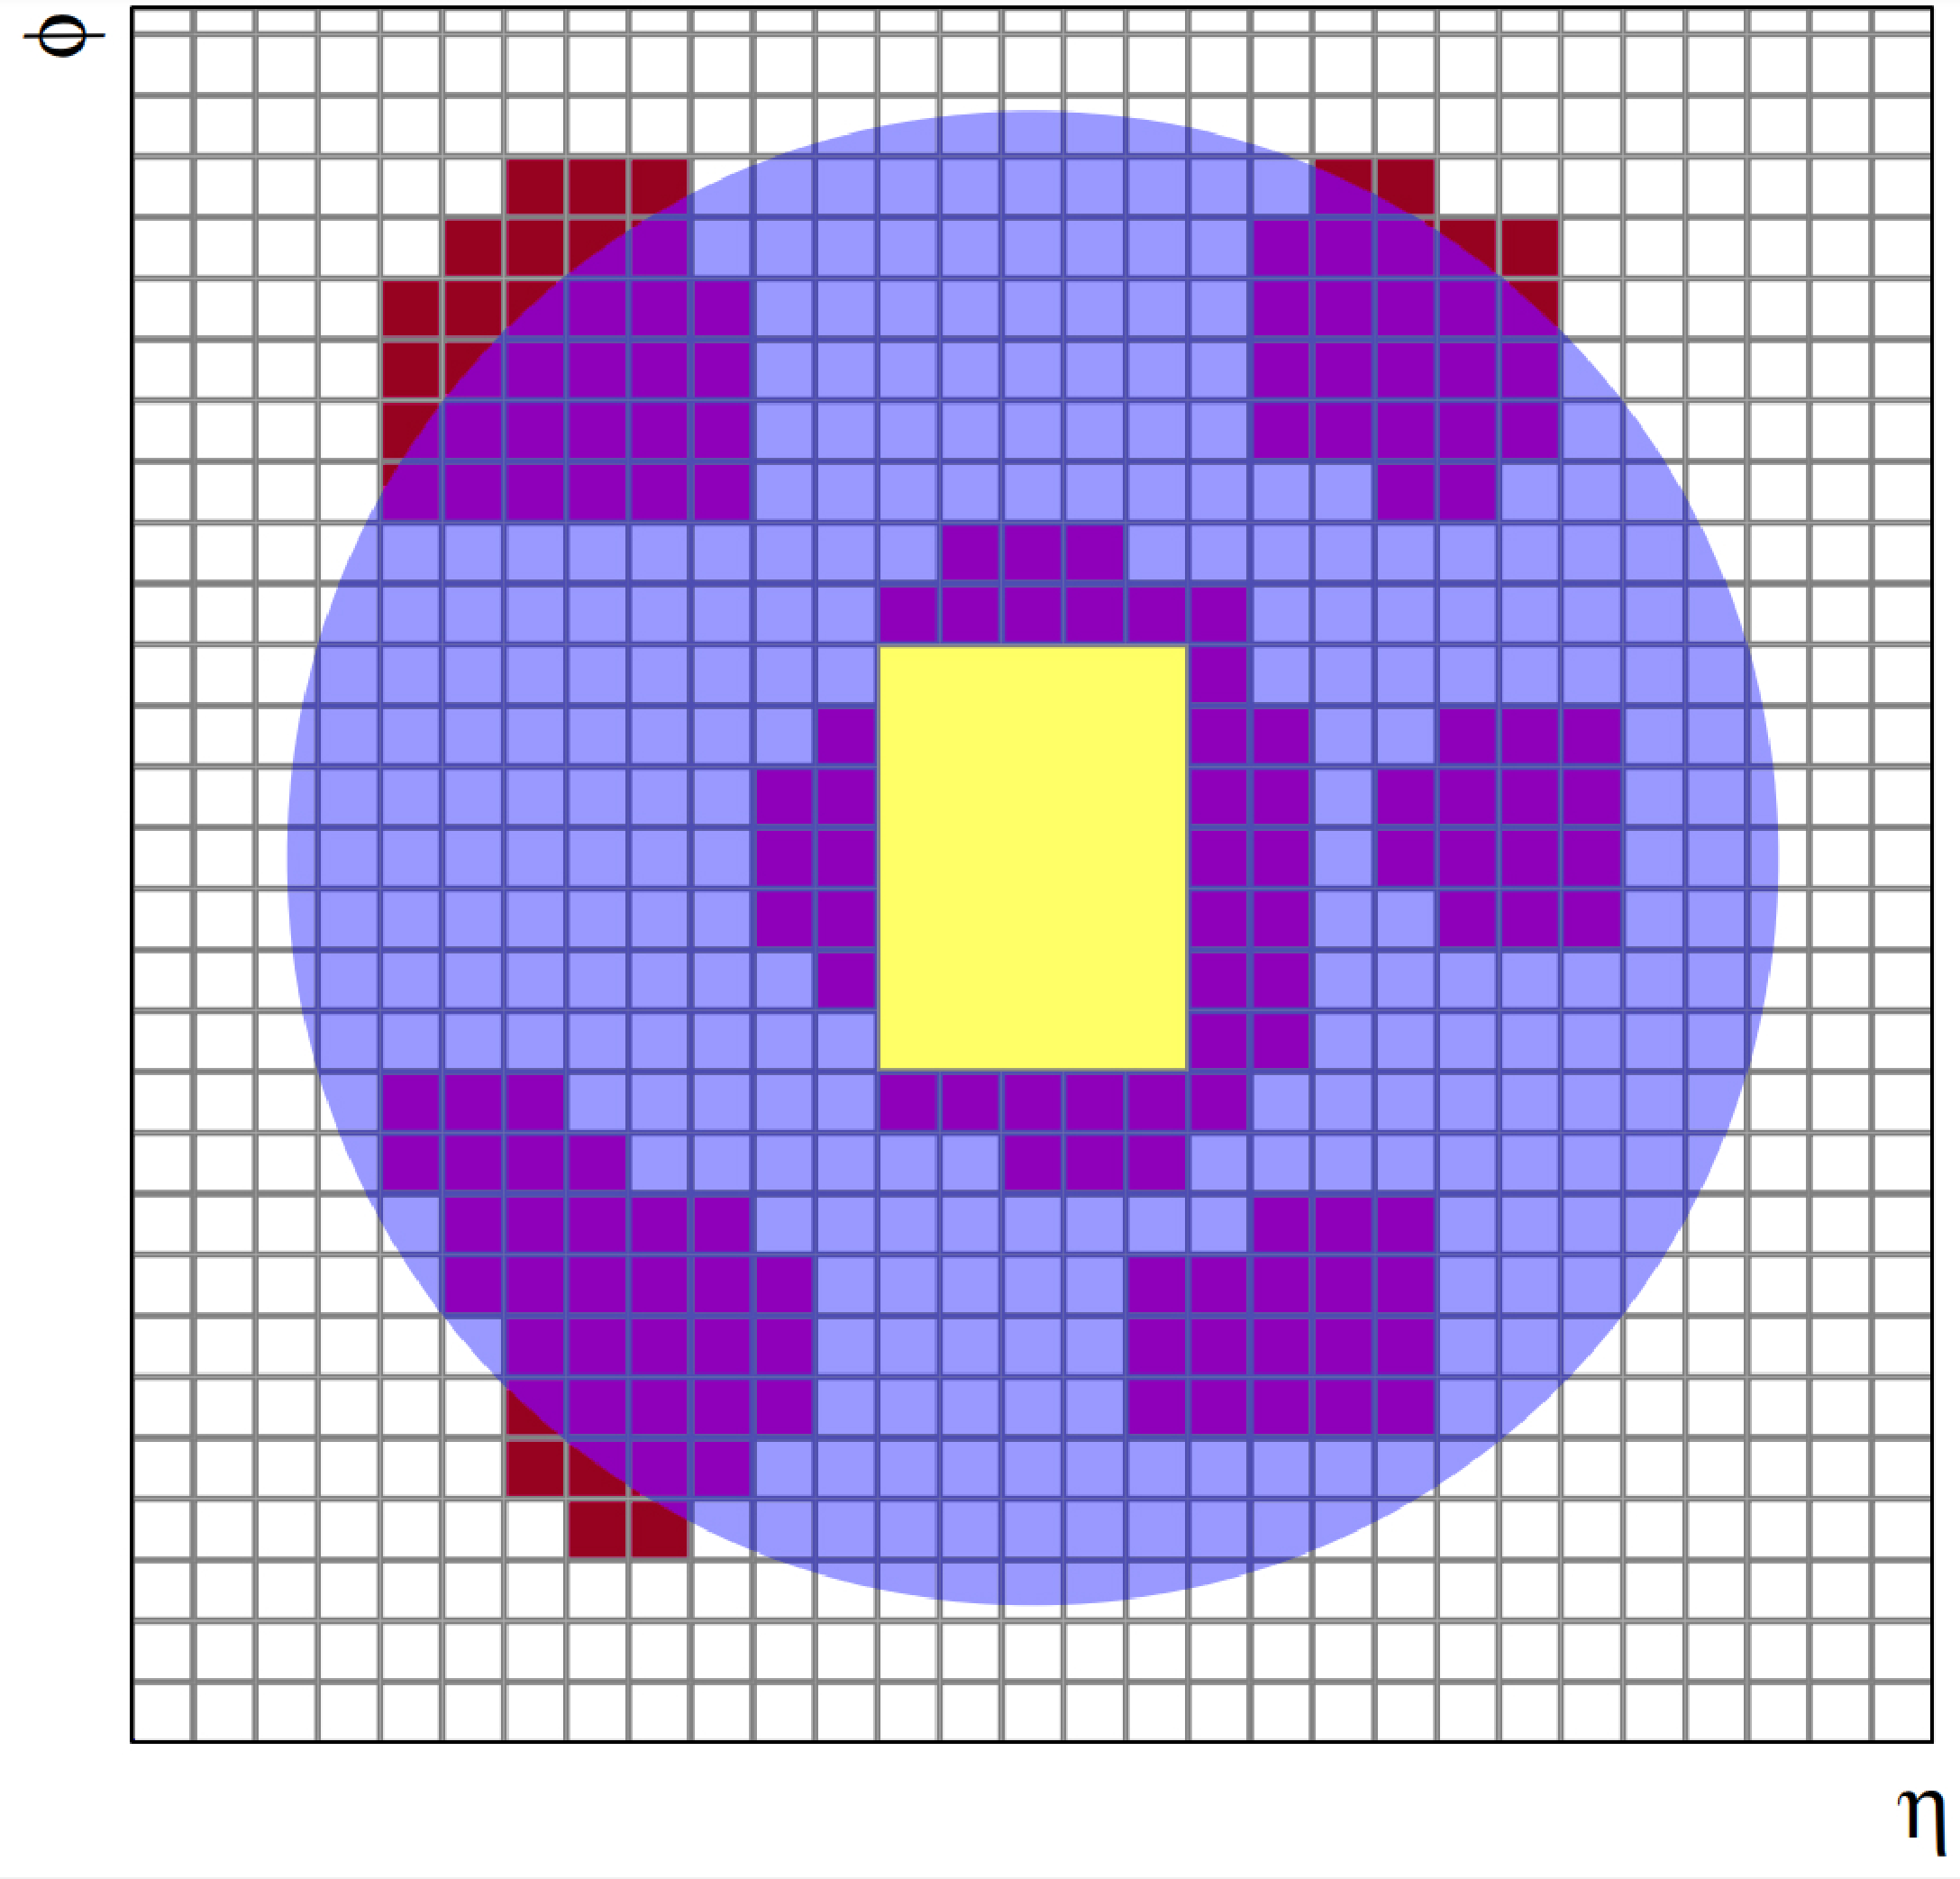
\includegraphics[width=\linewidth]{Assets/Images/electron_isol.pdf}
    \caption{Esquema del método de aislamiento calorimétrico de los electrones: la grilla representa las celdas de la segunda capa del ECAL en las direcciones $\eta$ y $\phi$. El candidato a electrón es ubicado en el centro del círculo azul, representando el cono de aislamiento. Todos los topo-clusters, representados en rojo, para los que sus baricentros intersecten el cono de aislamiento serán incluidos en $E_{T,\text{raw}}^{\text{iso}}$. La zona central en amarillo corresponde a las celdas sustraidas.}
    \label{fig:ch3:elec_isol}
\end{marginfigure}

El aislamiento calorimétrico es calculado a partir de las celdas en todos los calorímetros, ECAL y HCAL, definiendo un cono con un cierto radio $R$ (usualmente 0.2) centrado en el baricentro del cluster del objeto; la energía total contenida en todos los clusters cuyos baricentros intersecten el cono se denomina $E_{T,\text{raw}}^{\text{iso}}$. La contribución del propio electrón es sustraida, removiendo las celdas del \textit{core} en un rectángulo de $\Delta\eta \times \Delta\phi = 0.125 \times 0.175$ centrado en el baricentro del cluster principal, como podemos observar en la \cref{fig:ch3:elec_isol}. Se aplica una calibración para corregir las filtraciones de energía del \textit{core} en la zona de aislamiento y los efectos del \textit{pile-up}. La energía resultante,
\[ E_T^{\text{iso}} = E_{T,\text{raw}}^{\text{iso}} - E_{T,\text{core}} - E_{T,\text{leakage}} - E_{T,\text{pile-up}}, \]
se puede comparar con la energía transversa total del candidato a electrón.

Combinando ambos criterios de aislamiento y definiendo diferentes valores máximos de los parámetros $E_T^{\text{iso}}(\Delta R)/E_T$ y $p_T^{\text{iso}}(\Delta R)/p_T$ para distintos valores de $\Delta R$, se definen múltiples \textit{working points} para el aislamiento de los electrones. En el presente análisis se hace uso del criterio de aislamiento \texttt{FCLoose} para los electrones, definido como $E_T^{\text{iso}}(\Delta R < 0.2)/E_T < 0.2$ y $p_T^{\text{iso}}(\Delta R^{\text{var}} < 0.2)/p_T < 0.15$.,



\subsection{Muones}

Debido a su mínima interacción con la materia, los muones producidos en colisiones pp suelen atravesar todo el detector antes de proceder a decaer a electrones y neutrinos, luego de una pequeña vida media propia, de \SI{2.2}{\micro\second}. Si bien la mayor parte de las señales utilizadas en su reconstrucción provienen del MS, lo muones producen trazas identificables en el ID, e incluso pueden dejar pequeños depósitos de energía en los calorímetros (que a veces se utilizan para aumentar la cobertura en $\eta$ y la resolución de su $p_T$)~\cite{TheATLASCollaboration2016}.

\paragraph{Reconstrucción}

La reconstrucción de los muones se realiza primero de manera independiente en el ID y en el MS. Para los muones que han dejado trazas detectables en el ID, su reconstrucción es análoga al caso de los electrones (y cualquier otra partícula cargada).

La reconstrucción de trazas en el MS se realiza unificando patrones de interacciones, o \textit{hits}, en las distintas clases de cámaras de muones, hasta conformar segmentos. Los segmentos de múltiples capas son ajustados, conformando un primer conjunto de candidatos de muones físicos.

La aceptancia del ID y el MS es limitada en algunas regiones extremas de alto $\abs{\eta}$, por lo que se utiliza información complementaria de topo-clusters en los calorímetros.

A partir de una combinación de la información provista por estos tres métodos, los muones detectados por ATLAS pueden ser clasificados en cuatro categorías:
\begin{itemize}
    \item \textsc{Muones Extrapolados} (EM, \textit{Extrapolated muons}): su trayectoria se reconstruye solo utilizando trazas del MS, con trazas que atraviesen al menos dos capas del MS. Se pide un requerimiento \textit{loose} en su compatibilidad con el vértice original. Son utilizados para extender la cobertura en la región $2.5 < \abs{\eta} < 2.7$, no cubierta por el ID.
    \item \textsc{Muones Calorimétricos} (CT, \textit{Calorimeter-tagged muons}): Construidos a partir de una única traza en el ID y pequeños depósitos de energía en los calorímetros. No se utiliza información del MS, por lo que su pureza no suele ser buena. Están optimizados para $15 < p_T < \SI{100}{\GeV}$ en la región $\abs{\eta} < 0.1$, donde el MS está parcialmente instrumentado.
    \item \textsc{Muones Segmentados} (ST, \textit{Segment-tagged muons}): Conformados por una traza reconstruida en el ID, extrapolada y vinculada con al menos un segmento de traza en las cámaras MDT o CSC del MS. Los ST son utilizados para recuperar muones de bajo $p_T$ que solo atraviesan una capa del MS, o aparecen en una región con reducida aceptancia del MS.
    \item \textsc{Muones Combinados} (CB, \textit{Combined muons}): Obtenidos al combinar por medio de un re-ajuste global una traza reconstruida en el ID, con una traza reconstruida en el MS. Poseen la mayor resolución de $p_T$. La mayoría de los candidatos a muones se encuentran en esta categoría.
\end{itemize}

Si un muón es reconstruido bajo más de una categoría, entonces se priorizan en el siguiente órden: si comparten la misma traza del ID, se prefieren los CB, luego los ST y finalmente los CT. El solapamiento con muones ME se resuelve seleccionando las trazas con mejor ajuste y mayor número de \textit{hits}. En todos los casos, la energía es calibrada para tener en cuenta las pérdidas al atravesar los calorímetros. 


\paragraph{Identificación}

Para distinguir muones aislados de aquellos provenientes de procesos de fondo (principalmente del decaimiento de $\pi^\pm$ y $K^\pm$), se utilizan una serie de cortes de calidad. Al igual que en los electrones, se definen distintos \textit{working points}, de acuerdo a la eficiencia de aceptancia de la señal.

En nuestro análisis utilizamos el WP \textit{Medium}, que solo considera muones CB y EM para minimizar las incertezas sistemáticas asociadas a la reconstrucción y calibración. Los muones CB deben tener al menos 3 \textit{hits} en al menos 2 capas del MDT, excepto trazas en la región $\abs{\eta} < 0.1$, donde este requerimiento se reduce a 1 capa. Los muones EM deberán tener al menos tres capas en el MDT y CSC, y solo se utilizan para extender la cobertura por fuera del ID. Se aplica una selección simple de la compatibilidad entre las mediciones de momento entre el ID y el MS, para suprimir la contaminación por hadrones mal-identificados como muones.

\paragraph{Aislamiento}

Los muones cuentan con un procedimiento de aislamiento análogo al introducido en el caso de los electrones. En este análisis utilizamos el criterio de aislamiento \texttt{Loose\_VarRad} para los muones, definido como $E_T^{\text{iso}}(\Delta R < 0.2)/p_T < 0.3$ y $p_T^{\text{iso}}(\Delta R^{\text{var}} < 0.3)/p_T < 0.15$.




\subsection{Jets} \label{sec:ch3:jets}

Los \textit{jets}, o chorros de partículas, son el resultado de la hadronización de quarks y gluones generados en la dispersión dura, debido al principio de confinamiento de QCD descrito en la \cref{sec:ch1:SM:QCD}. Existen múltiples técnicas para realizar la reconstrucción, calibración y clasificación de jets, aunque casi todas comienzan por la producción de semillas de jets con el algoritmo anti-$k_t$.

\paragraph{Algoritmo anti-$k_t$}

El algoritmo anti-$k_t$ es un algoritmo iterativo utilizado en ATLAS para agrupar trazas del ID y topo-clusters reconstruidos en los calorímetros, conformando candidatos a jets. Es muy poco sensible a la radiación \textit{soft}, por lo que resulta ideal en las condiciones de elevado \textit{pile-up} en que se dan las interacciones en el LHC~\cite{Cacciari2008}.

El proceso comienza con la formación de un conjunto de semillas de jets, a partir de la selección de objetos con $p_T > \SI{7}{\GeV}$. Una vez obtenidas las semillas, comienza un proceso iterativo de cuatro pasos:
\begin{enumerate}
    \item Se identifica entre todos los objetos de la colección el par $(i, j)$ con el menor valor del parámetro de distancia
    \[ d_{ij} = \min\qty{p_{T,i}^{2p}, p_{T,j}^{2p}} \frac{\Delta R_{ij}^2}{R^2}, \]
    donde $p$ es un parámetro característico del algoritmo, y el parámetro $R$ influencia el radio de los jets resultantes (usualmente $R = 0.4$ en la reconstrucción estándar de jets). Se opta por $p = -1$, para priorizar los clusters de partículas \textit{hard}, tal que el jet crezca hacia el exterior de la semilla.
    \item Si $d_{ij}^{\text{min}}$ es menor a la distancia $d_{i,B} = p_{T,i}^{2p}$ entre el cluster $i$ y el haz, el cluster se convierte en un jet y se remueve de la colección.
    \item Si $d_{ij}^{\text{min}}$ es menor que $\min{p_{T,i}^{2p}, p_{T,j}^{2p}}$, los objetos son recombinados en un nuevo cluster con $p^\mu_{\text{new}} = p^\mu_i + p^\mu_j$.
    \item El procedimiento se repite hasta que no restan clusters en la colección.
\end{enumerate}


\paragraph{Reconstrucción e identificación}

Los jets reconstruidos en ATLAS y utilizados en los análisis se pueden clasificar en dos grandes categorías, dependiendo de la información suministrada al algoritmo anti-$k_t$. Aquellos que solo utilizan topo-clusters del calorímetro son conocidos como TopoJets, mientras que si se emplean también las trazas reconstruidas en el ID los jets reciben el nombre de PFlowJets, por el algoritmo ``Particle Flow'' utilizado para pre-procesar los topo-clusters. En este análisis solo se utilizan PFlowJets, por lo que procederemos a su descripción en las próximas líneas.

El algoritmo \textit{Particle Flow} (PF) permite combinar las mediciones en los calorímetros con las trazas reconstruidas en el ID, de mejor resolución en la determinación del momento, especialmente en el régimen de bajo $p_T$~\cites[-7em][]{TheATLASCollaboration2017a}[-3em][]{TheATLASCollaboration2018}. Su ejecución comienza vinculando trazas del ID con topo-clusters en los calorímetros, estimando la energía depositada en cada celda del ECAL y el HCAL por las partículas correspondientes a las trazas. La estimación es luego sustraida en cada celda, teniendo en cuenta la probabilidad de haber depositado energía en múltiples celdas y topo-clusters adyacentes. Finalmente, los topo-clusters cuya energía remanente se encuentra debajo del ruido de los detectores son removidos. Los topo-clusters sobrevivientes al algoritmo PF, junto con \textit{tracks} que satisfagan $\abs{z_0 \sin\theta} < \SI{2}{\milli\meter}$ (para suprimir el \textit{pile-up} de interacciones \textit{soft}) son utilizados como entradas del algoritmo anti-$k_t$.

El conjunto de jets reconstruidos es calibrado en un proceso de múltiples etapas, en el que se incluye una corrección al \textit{pile-up}, una corrección a la escala de energía basada en MC (\textit{Jet Energy Scale}) y una corrección final \textit{in-situ} aplicada solamente a los datos.

Para reducir la contaminación de jets provenientes de \textit{pile-up} en la reconstrucción, se utiliza una combinación multivariable llamada JVT, o \textit{Jet Vertex Tagger}, que utiliza las variables corrJVF\sidenote[][-17em]{\textit{Corrected Jet Vertex Fraction}, definida como
\begin{align*}\displaystyle
    &\text{corrJVF} = \\
    &\quad \frac{\sum_k p_{T}^{\text{trk}_k}(PV_0)}{\sum_l p_T^{\text{trk}_l}(PV_0) + \displaystyle \frac{\sum_{n \geq 1} \sum_l p_T^{\text{trk}_l}(PV_n)}{N_{\text{trk}}^{\text{PU}} \ k}},
\end{align*}
donde el numerador comprende una suma de los momentos transversos de todas las trazas provenientes del vértice primario, y el denominador una suma de los momentos transversos de las trazas de todos los vértices primarios (un vértice de dispersión \textit{hard} y otros vértices de \textit{pile-up}, estando estos últimos corregidos por un factor $k$ que considera el gradiente de $p_T^{\text{PU}}$ con respecto al número de trazas de \textit{pile-up} $N_{\text{trk}}^{PU}$, mitigando así una dependencia en el número total de vértices).
}, que mide la probabilidad de que un jet se haya originado en un vértice particular, y $R_{p_T}$, que combina información de los calorímetros y trazas del ID para cada jet\sidenote[][-0.4em]{Definida como \[ R_{p_T} = \frac{\sum_k p_T^{\text{trk}_k} (PV_0)}{p_T^{\text{jet}}}. \]}.


\paragraph{Procedimiento de $b$-Tagging}

Los jets originados en la hadronización de quarks $b$ pueden ser identificados utilizando algoritmos que exploten algunas de sus características distintivas. Estas incluyen su larga vida media, su gran masa --en comparación con la masa quarks livianos-- y la alta multiplicidad del decaimiento. En particular, la vida media de $\sim \SI{1.5}{\pico\second}$, significativamente mayor a la de otros quarks livianos, les permite desplazarse, moviendo su vértice de decaimiento algunos milímetros del vértice primario donde se ha producido el jet~\cite{ATL-PHYS-PUB-2017-013, ATL-PHYS-PUB-2014-014}, como podemos observar en la \cref{fig:ch3:secondary_vertex}.

\begin{marginfigure}
    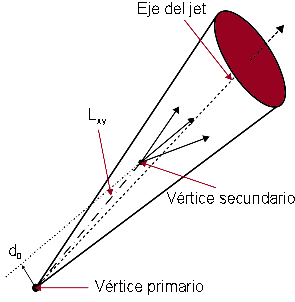
\includegraphics[width=\linewidth]{Assets/Images/secondary_vertex.pdf}
    \caption{Decaimiento de un quark $b$ hadronizado dentro de un jet, resultando en un vértice secundario con tres trazas de partículas cargadas, desplazado una distancia $L_{xy}$ en el plano transverso.}
    \label{fig:ch3:secondary_vertex}
\end{marginfigure}

En nuestro análisis, un jet anti-$k_t$ de $R = 0.4$ es etiquetado un BJet si pasa los requerimientos del algoritmo de \textit{$b$-Tagging} MV2c10~\cite{Aad2019}, en el WP de 85\% de eficiencia de identificación correcta. Para ser considerados candidatos $b$-jets, los jets también deberán satisfacer las selecciones $p_T > \SI{20}{\GeV}$, $\abs{\eta} < 2.5$, y haber pasado el corte correspondiente en JVT. Este algoritmo clasificador utiliza un discriminante BDT (\textit{Boosted Decision Tree}), cuyo principio general de funcionamiento se explicará en la \cref{sec:ch3:ditaus}.



\subsection{Taus} \label{sec:ch3:single-taus}

La reconstrucción convencional de taus decayendo hadrónicamente se realiza en ATLAS combinando información del ID y de los calorímetros, asociando a cada candidato de \thad un jet anti-$k_t$ de parámetro $R = 0.4$~\cite{Hubner2018}. Los jets deberán pasar los cortes de calidad cinemáticos $p_T > \SI{10}{\GeV}$, $\abs{\eta} < 1.37$ o $1.52 < \abs{\eta} < 2.5$ (removiendo la región de transición) y además ser vetados por un algoritmo de $b$-tagging en el WP de 77\% de eficiencia.

Debido a la cinemática de los hadrones resultantes del decaimiento, se espera contener a las trazas de mayor energía en la región central (\textit{core}) $0 < \Delta R < 0.2$ en el caso de objetos \ttau físicos (significativamente menor al diámetro de los jets de QCD producidos por quarks o gluones descritos en la sección anterior), por lo que el $p_T$ calibrado del objeto se determina con los depósitos calorimétricos en esta región. En el anillo externo $0.2 < \Delta R < 0.4$ no se espera la presencia de partículas físicas, por lo que es considerado una región de aislamiento.

El número de trazas en la región central clasifica al objeto como un candidato a \thad \textit{1-prong}, \textit{3-prong}, o \textit{multi-prong}, siendo los primeros dos identificados con los decaimientos hadrónicos más comunes del tau.

Una vez recuperado el vértice de decaimiento del \ttau (utilizando una variante del JVT introducido en la \cref{sec:ch3:jets}, seleccionando entre los candidatos finales el de mayor $\sum p_T^2$), la información del jet en sus distintas regiones es introducida a un BDT, donde los \thad \textit{1-prong} y \textit{3-prong} son identificados separadamente.


{ % I have to remove the "Global" \smallcapslsstyle{50}, because it ruins the MET math text
\titleformat{\subsection}%
  [hang]% shape
  {\normalfont\color{darkgray}\Large}% format applied to label+text
  {\large\smallcapslsstyle{50}{\thesubsection}}% label
  {1em}% horizontal separation between label and title body
  {}% before the title body
  []% after the title body
\subsection{{\lsstyle\scshape\MakeTextLowercase{Energía Transversa Faltante}} (\texorpdfstring{$E_T^{\text{miss}}$}{MET})}
} \label{sec:ch3:met}

La conservación del momento en el plano transverso, introducida en la \cref{sec:ch2:atlas_coordinates}, garantiza que la suma de los momentos transversos de todos los productos de la colisión sea nula. Sin embargo, la presencia de partículas no-interactuantes o débilmente interactuantes (y, por lo tanto, no detectadas), puede producir desbalances en el cálculo, resultando en un momento transverso faltante $p_T^{\text{miss}}$. Esto puede ser asociado con neutrinos en el estado final de la interacción, aunque también puede provenir de otras partículas débilmente interactuantes fuera del SM. El momento transverso faltante puede tener también una componente ``falsa'', originada por partículas que escapen la aceptancia del detector, o por partículas con una reconstrucción incompleta como consecuencia de la limitada aceptancia del detector, de su resolución finita, las regiones parcialmente instrumentadas, o alguna fuente de ruido.

El momento faltante en el plano transverso es reconstruido como la magnitud negativa de la suma vectorial de los momentos en el plano transversal de todas las partículas reconstruidas y un término que tiene en cuenta las contribuciones de objetos \textit{soft}. En nuestro análisis, considerando las partículas de interés en el estado final,
\[ \vb{p}_T^{\text{miss}} = \vb{p}_T^{\text{miss, }e} + \vb{p}_T^{\text{miss, }\mu} + \vb{p}_T^{\text{miss, jets}} + \vb{p}_T^{\text{miss, soft}}. \]
Puede ocurrir que un conjunto de señales en el detector sean reconstruidas e identificadas erróneamente como múltiples tipos de partículas, resultando en un doble-conteo de las contribuciones al $\vb{p}_T^{\text{miss}}$. En estos casos, se aplica un procedimiento de eliminación de superposiciones (OR, \textit{Overlap Removal}), priorizando solo uno de los candidatos de partículas~\cite[-9em][]{TheATLASCollaboration2018}.

En particular, debido al gran número de jets de \textit{pile-up} producidos en cada evento, el término $p_T^{\text{miss, jets}}$ solo considera jets anti-$k_t$ $R = 0.4$ de momento transverso $p_T > \SI{30}{\GeV}$ y que satisfagan el criterio adicional $JVT > 0.64$ para los jets con $p_T < \SI{60}{\GeV}$.

El término $p_T^{\text{miss, soft}}$ tiene como objetivo incluir las partículas de bajo $p_T$ que no hayan sido asociadas a los objetos principales \textit{hard} del evento. Se construye a partir de trazas con $p_T > \SI{0.4}{\GeV}$ y $\abs{\eta} < 2.5$. Para reducir contribuciones de \textit{pile-up}, se requiere que las trazas sean compatibles con el vértice primario, imponiendo cortes de calidad en los parámetros de impacto y en los \textit{hits} en el SCT y el detector de Píxeles.

El impulso total transverso faltante se define entonces como $p_T^{\text{miss}} = \sqrt{\qty(p_x^{\text{miss}})^2 + \qty(p_y^{\text{miss}})^2}$. Justificados en las asociaciones que podemos hacer entre el momento transverso y la energía transversa que desarrollamos en la \cref{sec:ch2:atlas_coordinates}, podemos entonces definir la energía transversa faltante $E_T^{\text{miss}}$ y su dirección azimutal $\phi^{\text{miss}}$ como:
\[ E_T^{\text{miss}} = \norm{\vb{p}_T^{\text{miss}}} \quad \text{y} \quad \phi^{\text{miss}} = \arctan(\frac{p_y^{\text{miss}}}{p_x^{\text{miss}}}). \]






\section{Los objetos DiTau} \label{sec:ch3:ditaus}

Como hemos introducido en la \cref{sec:ch1:ttX_phenomenology:signal}, debido a la elevada masa del par $t\bar{t}$, la naturaleza CP-odd y la baja masa del escalar $X$, la partícula $X$ será producida con un gran \textit{boost}. En consecuencia, los \ttaus en el estado final de los eventos $t\bar{t}(X\to\tau\tau)$ tendrán una reducida separación angular $\Delta R$. Esto puede observarse claramente en las distribuciones cinemáticas presentadas en la \cref{fig:ch3:ditau:truth:dR}, donde la distancia angular entre los \thad en partículas $X$ de \SI{20}{\GeV} resulta en su mayoría $\Delta R < 1$. 

\begin{marginfigure}[-53em]
    \subfloat[][\label{fig:ch3:ditau:truth:dR}]{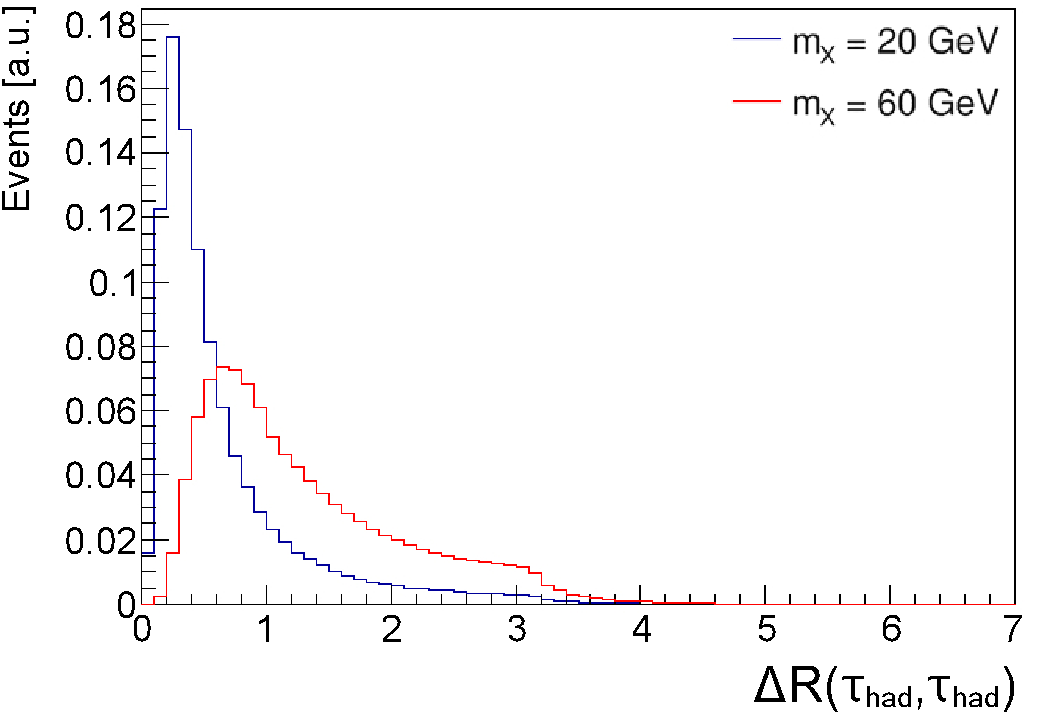
\includegraphics[width=0.99\marginparwidth]{Assets/Plots/DiTau/Truth/h_truth-tau_deltaR.pdf}}\\
    \subfloat[][\label{fig:ch3:ditau:truth:lead_pt}]{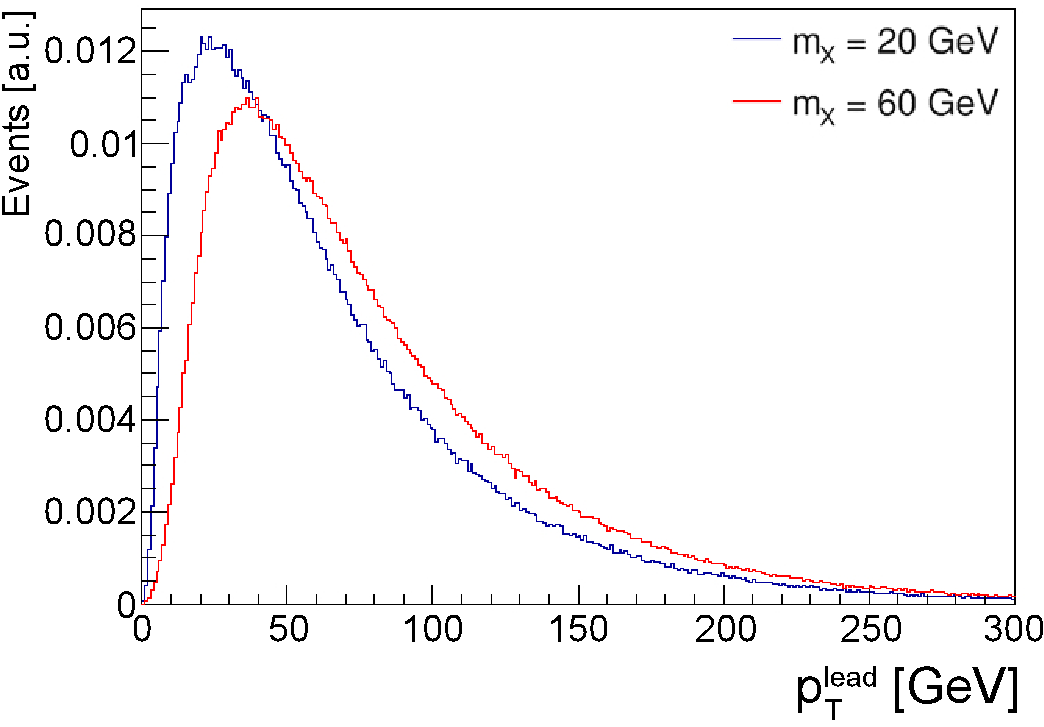
\includegraphics[width=0.99\marginparwidth]{Assets/Plots/DiTau/Truth/h_truth-tau_pt-lead.pdf}}\\
    \subfloat[][\label{fig:ch3:ditau:truth:subl_pt}]{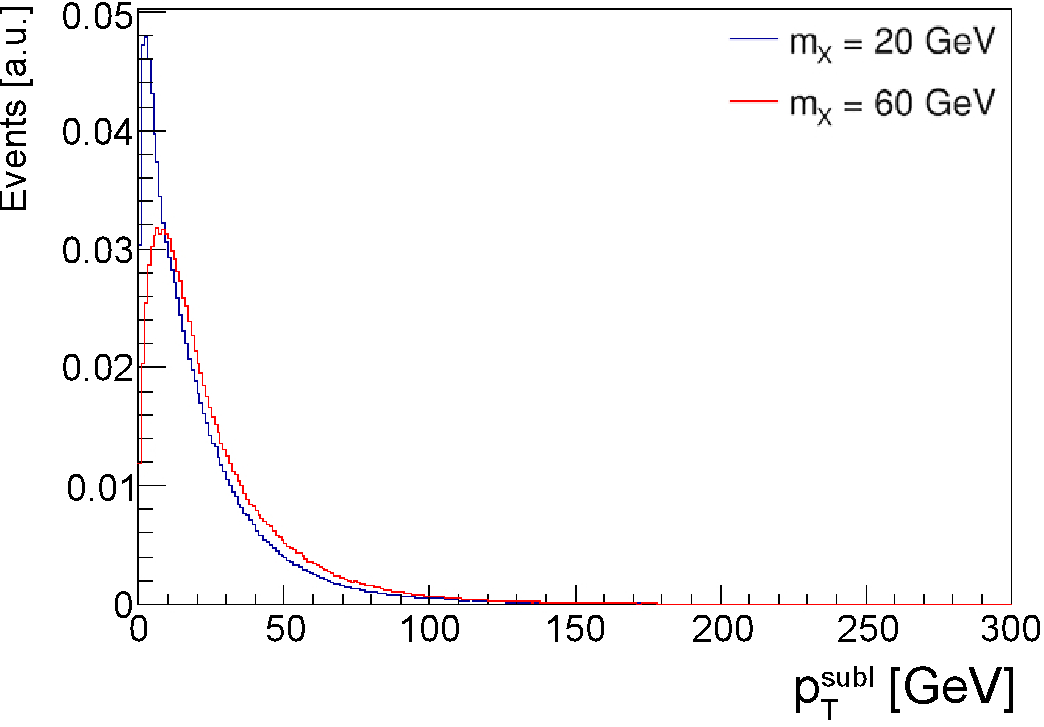
\includegraphics[width=0.99\marginparwidth]{Assets/Plots/DiTau/Truth/h_truth-tau_pt-subl.pdf}}
    \caption{Distribuciones de la separación angular $\Delta R$ \subref{fig:ch3:ditau:truth:dR}, $p_T$ de los $\tau_{\text{had}}$ \textit{leading} \subref{fig:ch3:ditau:truth:lead_pt} y \textit{subleading} \subref{fig:ch3:ditau:truth:subl_pt} producidos por el decaimiento de un pseudoescalar $X$ de \num{20} y \SI{60}{\GeV}.}
    \label{fig:ch3:ditau:truth}
\end{marginfigure}

Si intentáramos realizar el análisis de la forma convencional, tratando a los \ttaus en el estado final de la interacción como objetos \thad individuales como fue descrito en \ref{sec:ch3:single-taus}, la reconstrucción e identificación de los \thads fallaría progresivamente conforme se reduce su separación angular $\Delta R$. En el régimen $0.4 < \Delta R < 0.6$, la región central de uno de los \thad (${\Delta R < 0.2}$ del baricentro del jet asociado a cada \thad) comienza a solaparse con la zona de aislamiento del otro \thad ($0.2 < \Delta R < 0.4$), por lo que la eficiencia de identificación comienza a disminuir significativamente. Si la separación es aún menor ($\Delta R < 0.4$) ambas regiones centrales se solapan, por lo que se produce una falla también en su reconstrucción. Por este motivo, el uso de objetos tau individuales es inadecuada para análisis en el régimen \textit{boosteado}.

Para contrarrestar estas limitaciones, se ha optado por emplear un nuevo método de reconstrucción e identificación utilizando técnicas de sub-estructura de jets~\cite{Han2017} en un único objeto \textit{DiTau}, reconstruido como un único jet de mayor radio, conteniendo en su interior al par de \thads boosteados. Este método fue introducido inicialmente para el estudio de eventos con decaimientos boosteados $h\to\tau\tau$ del bosón de Higgs~\cite{Kirchmeier2015}, aunque nunca antes había sido aplicado a bosones de masa inferior a $\SI{100}{\GeV}$. En su versión original, los objetos DiTau ya forman parte de la producción estándar de AODs en ATLAS, habiendo sido incorporados al framework ATHENA del experimento. Sin embargo, su reconstrucción supone un $p_T > \SI{300}{\GeV}$ para el sistema de taus, por lo que deben ser reimplementados para ser aplicables al presente análisis.

A continuación describiremos la topología de los objetos DiTau y los nuevos procedimientos de reconstrucción e identificación de estos nuevos objetos en el rango de bajas masas.



\subsection{Reconstrucción}

La reconstrucción de los objetos DiTau comienza con la producción de 1 jet anti-$k_t$ con parámetro de radio $R = 1$, utilizando información de los calorímetros y trazas reconstruidas en el ID preprocesadas por el algoritmo \textit{Particle Flow}, que fue descrito en \ref{sec:ch3:jets}. Deberá tener un momento transverso $p_T > \SI{50}{\GeV}$, esperando que contenga todos los productos finales del decaimiento de los dos \thad.

\begin{marginfigure}[12em]
    \subfloat[][\label{fig:ch3:ditau:diagram:tracks}]{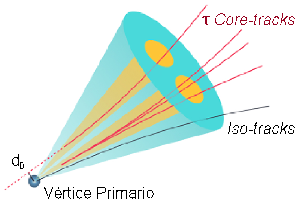
\includegraphics[width=0.99\marginparwidth]{Assets/Images/DiTau/DiTau_Reco.pdf}}\\
    \subfloat[][\label{fig:ch3:ditau:diagram:topology}]{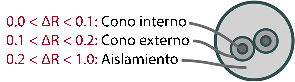
\includegraphics[width=0.99\marginparwidth]{Assets/Images/DiTau/ditau_diagram.pdf}}
    \caption[Esquema de un objeto DiTau: topología y disposición de trazas]{Esquema de un objeto DiTau. Topología del objeto \subref{fig:ch3:ditau:diagram:topology}; los conos internos de los dos subjets principales representan al par de \thads individuales. Disposición de trazas en las distintas regiones del objeto \subref{fig:ch3:ditau:diagram:tracks}.}
    \label{fig:ch3:ditau:diagram}
\end{marginfigure}

La subestructura del objeto DiTau es capturada por subjets PFlow anti-$k_t$ con $R = 0.2$, reconstruidos en el interior del jet $R = 1$. Se requiere que los candidatos contengan al menos $2$ subjets, cada uno con al menos $1$ \textit{track} asociado. Al contar con solo 2 \thad físicos, se espera que la mayor parte de la energía depositada se encuentre en los 2 subjets más energéticos, llamados \textit{leading} y \textit{subleading} (L y S, respectivamente). La región $\Delta R < 0.1$ del baricentro de cada subjet (\cref{fig:ch3:ditau:diagram}) recibe el nombre de \textit{cono interno} (\textit{core}), donde se esperan los mayores depósitos de energía. Por el contrario, la zona por fuera de los subjets LyS es considerada una región de aislamiento (\textit{isolation}), donde se suponen depósitos mucho menores, y muy pocas (o ninguna) traza, como podemos observar en la \cref{fig:ch3:ditau:diagram:tracks}.

La asociación de un vértice de producción del objeto DiTau se realiza por medio del algoritmo TJVA (\textit{Tau Jet Vertex Asociation}), similar al algoritmo utilizado para determinar el vértice de los \thad individuales. Se utilizan solo las trazas de los subjets LyS, sumando el $p_T$ de todas las trazas compatibles con todos los vértices posibles; el vértice con mayor $\sum p_T^2$ será considerado como vértice primario del objeto DiTau.

Finalmente, se realiza una selección definitiva de las trazas a incluir en el objeto. Los \textit{tracks} deberán satisfacer $p_T > \SI{1}{\GeV}$, $d_0 < \SI{1.0}{\milli\meter}$, $\abs{z_0 \sin\theta} < \SI{1.5}{\milli\meter}$ y haber realizado al menos 7 \textit{hits} en el detector de Píxeles y SCT, con al menos 2 de ellos en el primer subdetector. Esta selección está diseñada para maximizar la fracción de \thads \textit{1-prong} y \textit{3-prong} reconstruidos con el correcto número de \textit{tracks}, pudiendo entonces identificar su tipo de decaimiento.

\begin{marginfigure}
    \subfloat[][\label{fig:ch3:ditau:topo_plots:lead}]{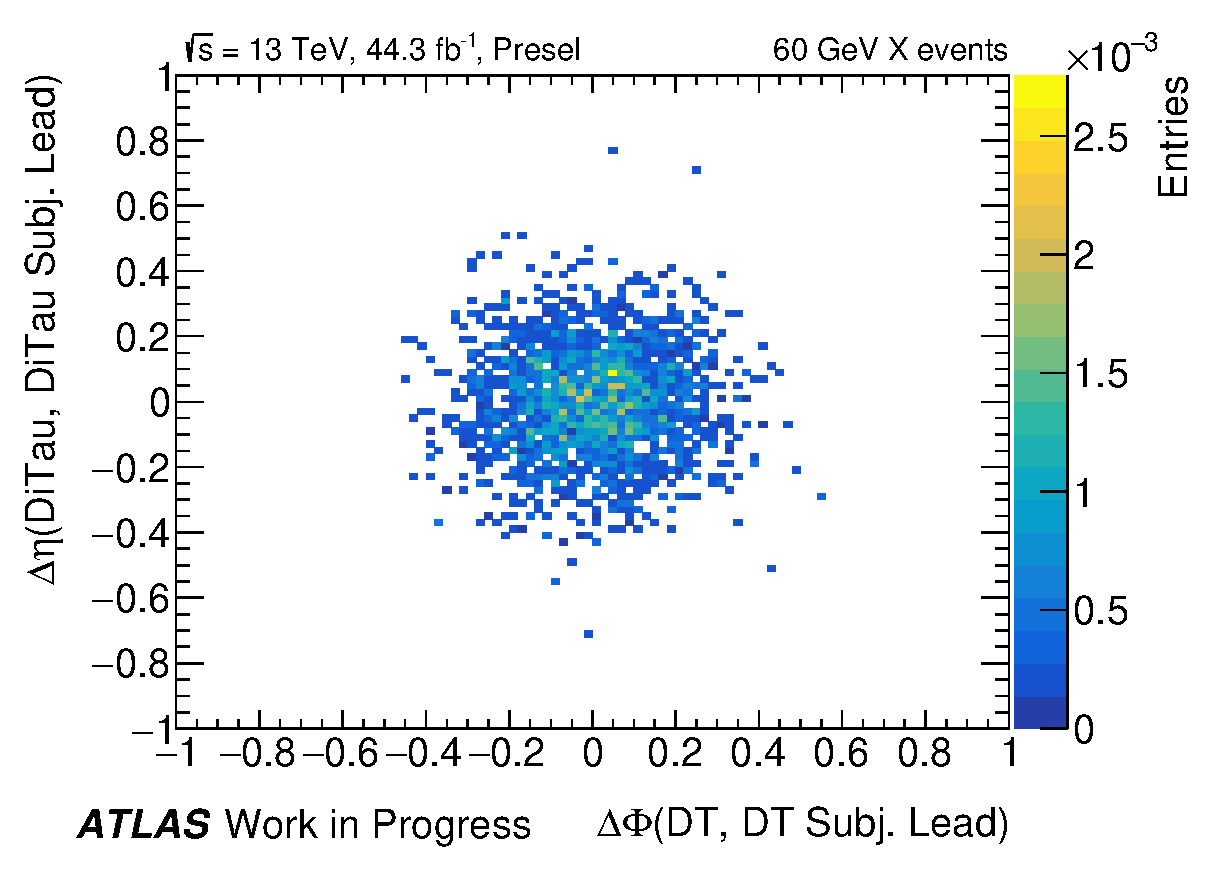
\includegraphics[width=\marginparwidth]{Assets/Plots/DiTau/Presel/Signal_TMH/h_mc16d_60_ditau_subj_lead_ditau_dphi_deta.eps}}\\
    \subfloat[][\label{fig:ch3:ditau:topo_plots:subl}]{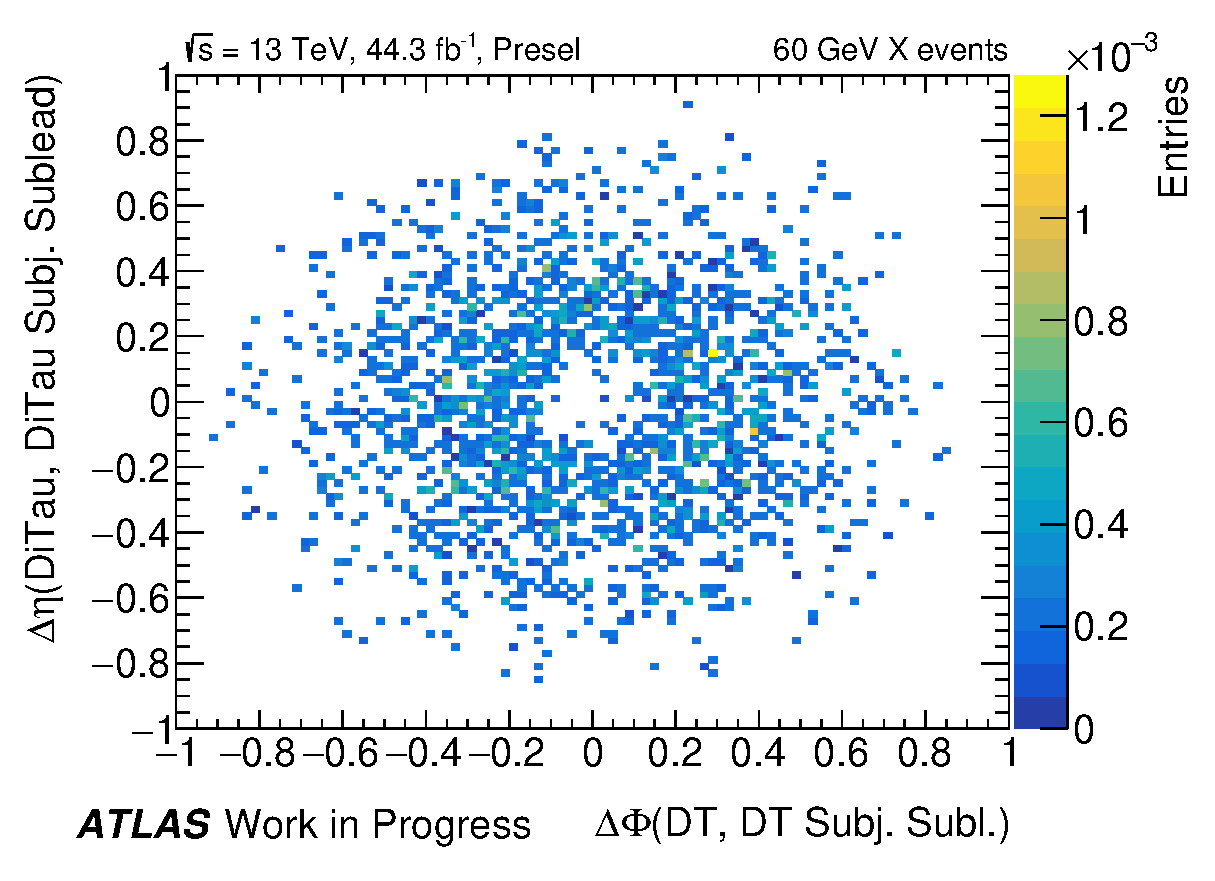
\includegraphics[width=\marginparwidth]{Assets/Plots/DiTau/Presel/Signal_TMH/h_mc16d_60_ditau_subj_subl_ditau_dphi_deta.eps}}
    \caption{Topología reconstruida de objetos DiTau (DT) \textit{truth} en una muestra de señal de \SI{60}{\GeV}: distribuciones de posición de los subjets \textit{leading} \subref{fig:ch3:ditau:topo_plots:lead} y \textit{subleading} \subref{fig:ch3:ditau:topo_plots:subl}.}
    \label{fig:ch3:ditau:topo_plots}
\end{marginfigure}

El cuadrimomento asignado al objeto DiTau corresponde al subsistema de subjets \textit{leading} y \textit{subleading}, es decir, $p^\mu_{\text{DiTau}} = p^\mu_{\text{lead}} + p^\mu_{\text{subl}}$. Los objetos reciben una calibración de energía (TES, \textit{Tau Energy Scale}), en donde se corrige su $p_T$ para mitigar el efecto del \textit{pile-up} e incluir la calibración de los detectores~\citeonly{ATLAS-CONF-2012-054}. Esta calibración se realiza en dos etapas:
\begin{equation}
    p_T^{\text{corr}} = p_T^{\text{reco}} - A(\abs{\eta}) N_{PV}, \quad p_T^{\text{calib}} = \frac{p_T^{\text{corr}}}{R(p_T^{\text{corr}}, \abs{\eta}, N_{\text{prong}})}, \label{eq:ch3:ditau:energy_cal}
\end{equation}
siendo $p_T^{\text{calib}}$ la magnitud final calibrada. Los factores de calibración $A(\abs{\eta})$ y $R(p_T^{\text{corr}}, \abs{\eta}, N_{\text{prong}})$ representan la corrección de \textit{pile-up} (donde $N_{PV}$ es el número de vértices primarios identificados en el evento) y la función respuesta del detector (dependiente de la energía, la región donde se detectó el objeto DiTau y el número de componentes hadrónicos reconstruidos en el decaimiento de cada $\tau_{\text{had}}$). La calibración se realiza a partir de simulaciones MC, utilizando objetos DiTau TM. La calibración en energía no ha sido incluida en los resultados del presente trabajo, encontrándose aún pendiente de validación.

Es importante recordar que, debido a la producción de neutrinos en el decaimiento hadrónico de los leptones \ttau, la masa invariante y energía total identificadas con el objeto DiTau no se corresponderá directamente con la masa y energía del sistema físico de dos \ttaus.

En general, el subjet \textit{leading} definirá la dirección del objeto DiTau, encontrándose casi siempre próximo a su baricentro. En el plano $\eta-\phi$, estos subjets más energéticos formarán un cúmulo circular, en la mayoría de los casos con $\Delta R < 0.2$, como podemos observar en la \cref{fig:ch3:ditau:topo_plots} para eventos de señal de \SI{60}{\GeV}. Por el contrario, los subjets \textit{subleading} forman un anillo, de mayor densidad en $0.2 < \Delta R < 0.4$ del baricentro del jet $R = 1$ del DiTau. Al contener una energía significativamente menor, como notamos en la \cref{fig:ch3:ditau:truth:subl_pt}, estos últimos objetos no tienen una fuerte injerencia en la orientación del DiTau.

La reconstrucción del objeto DiTau por medio de esta técnica resulta en las eficiencias exhibidas en la \cref{fig:ch3:ditau:reco_efficiency}.


\begin{marginfigure}[-15em]
    \subfloat[][\label{fig:ch3:ditau:reco_efficiency:pt}]{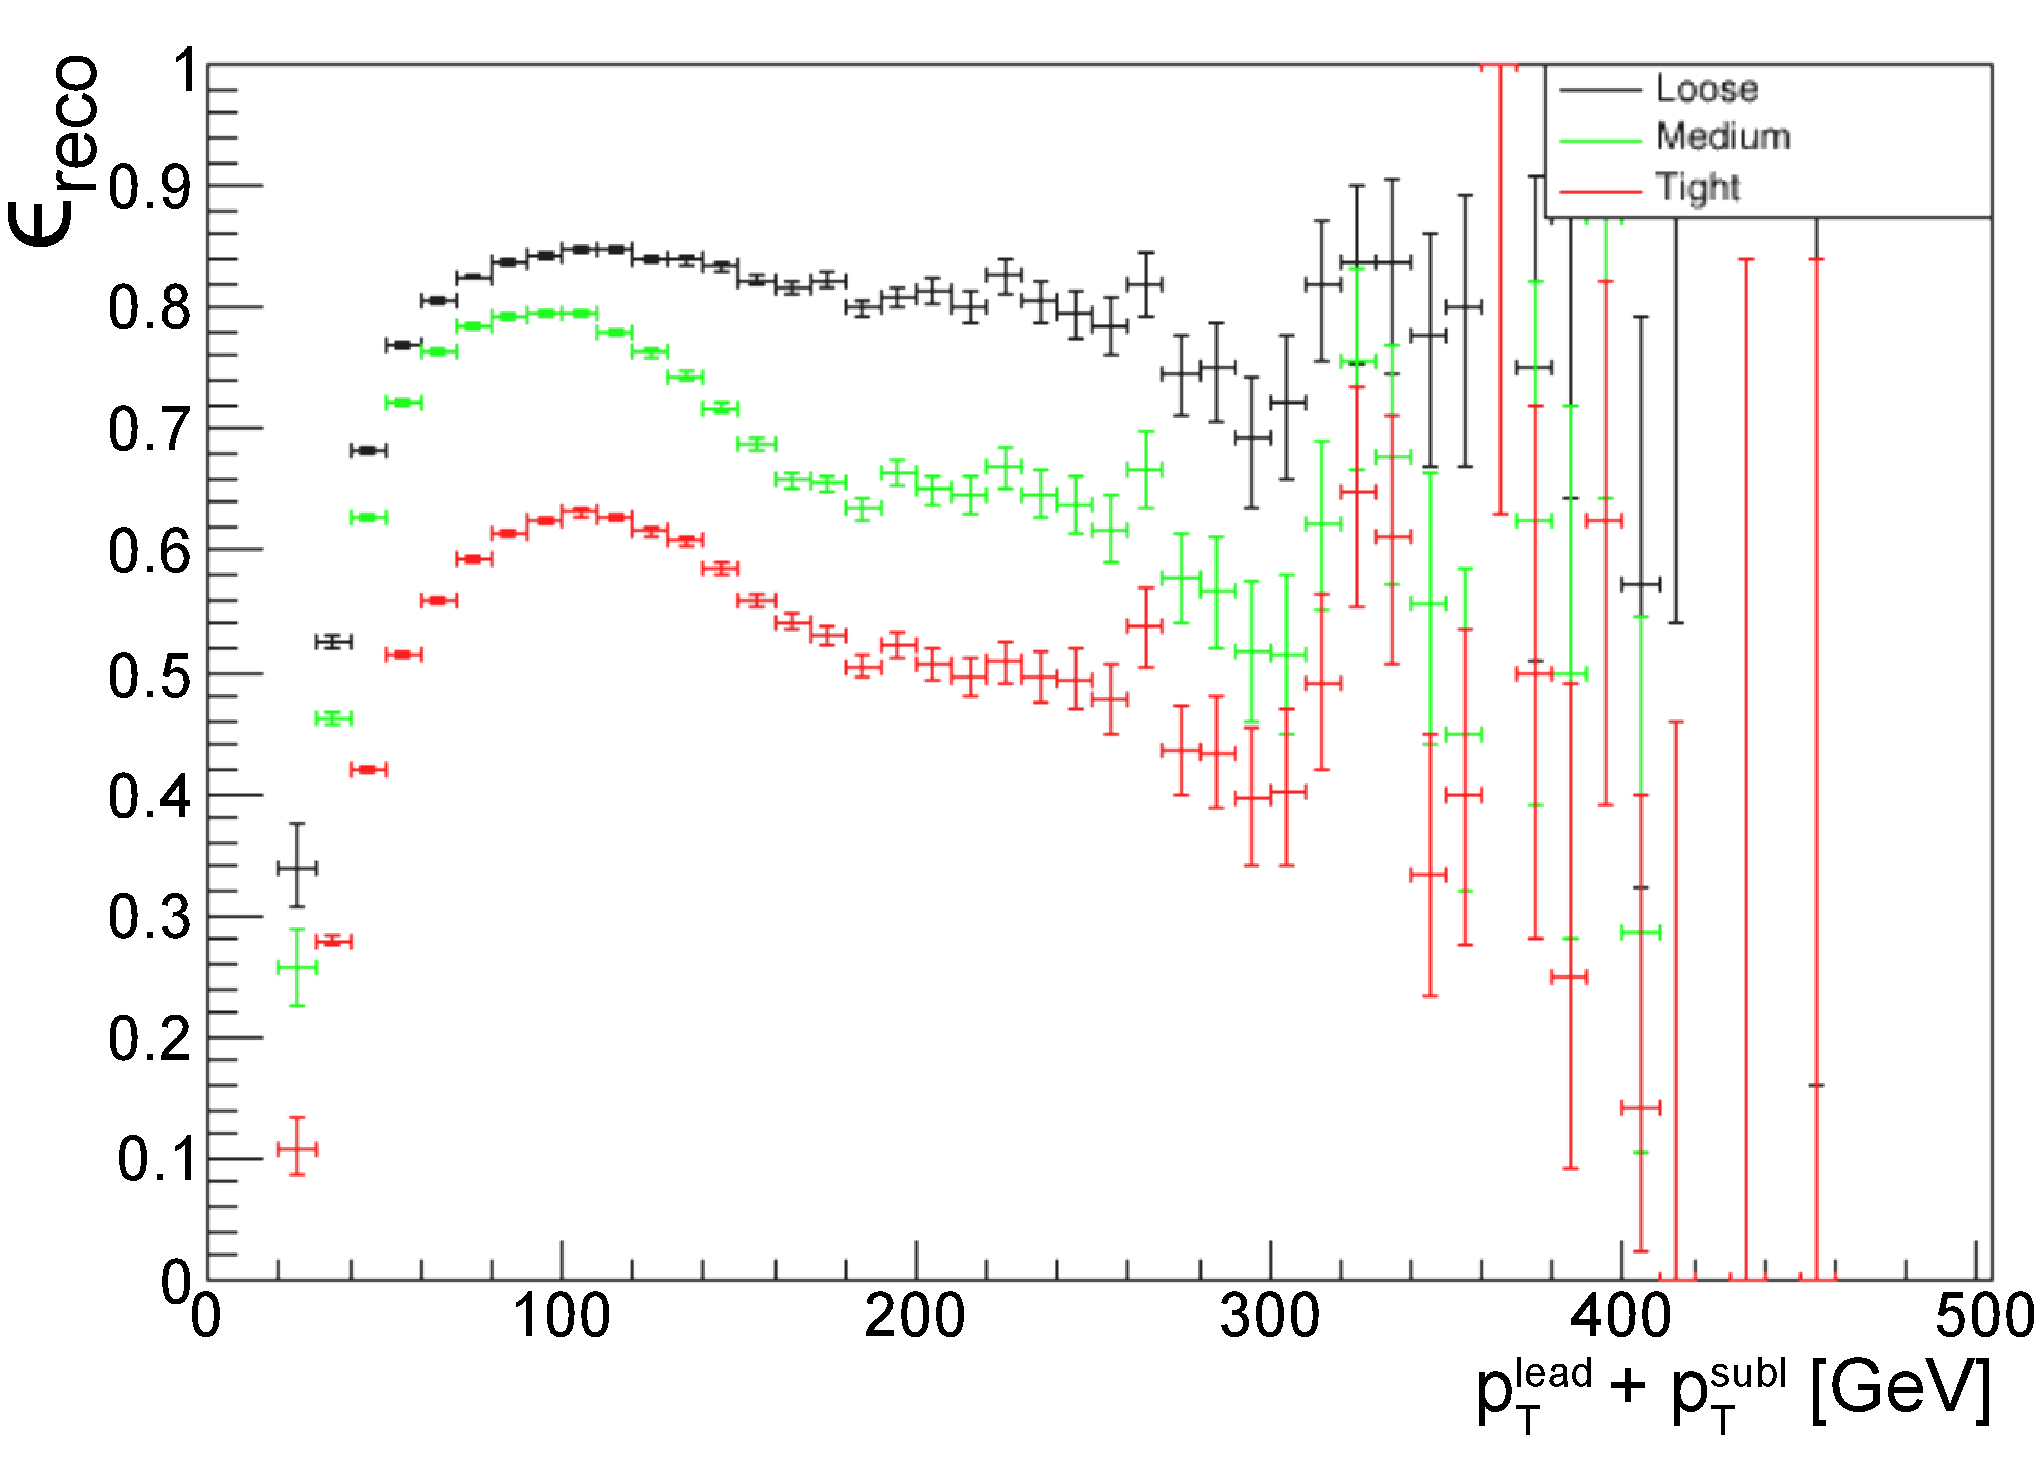
\includegraphics[width=0.99\marginparwidth]{Assets/Plots/DiTau/Reco/efficiency_pt.pdf}}\\
    \subfloat[][\label{fig:ch3:ditau:reco_efficiency:dR}]{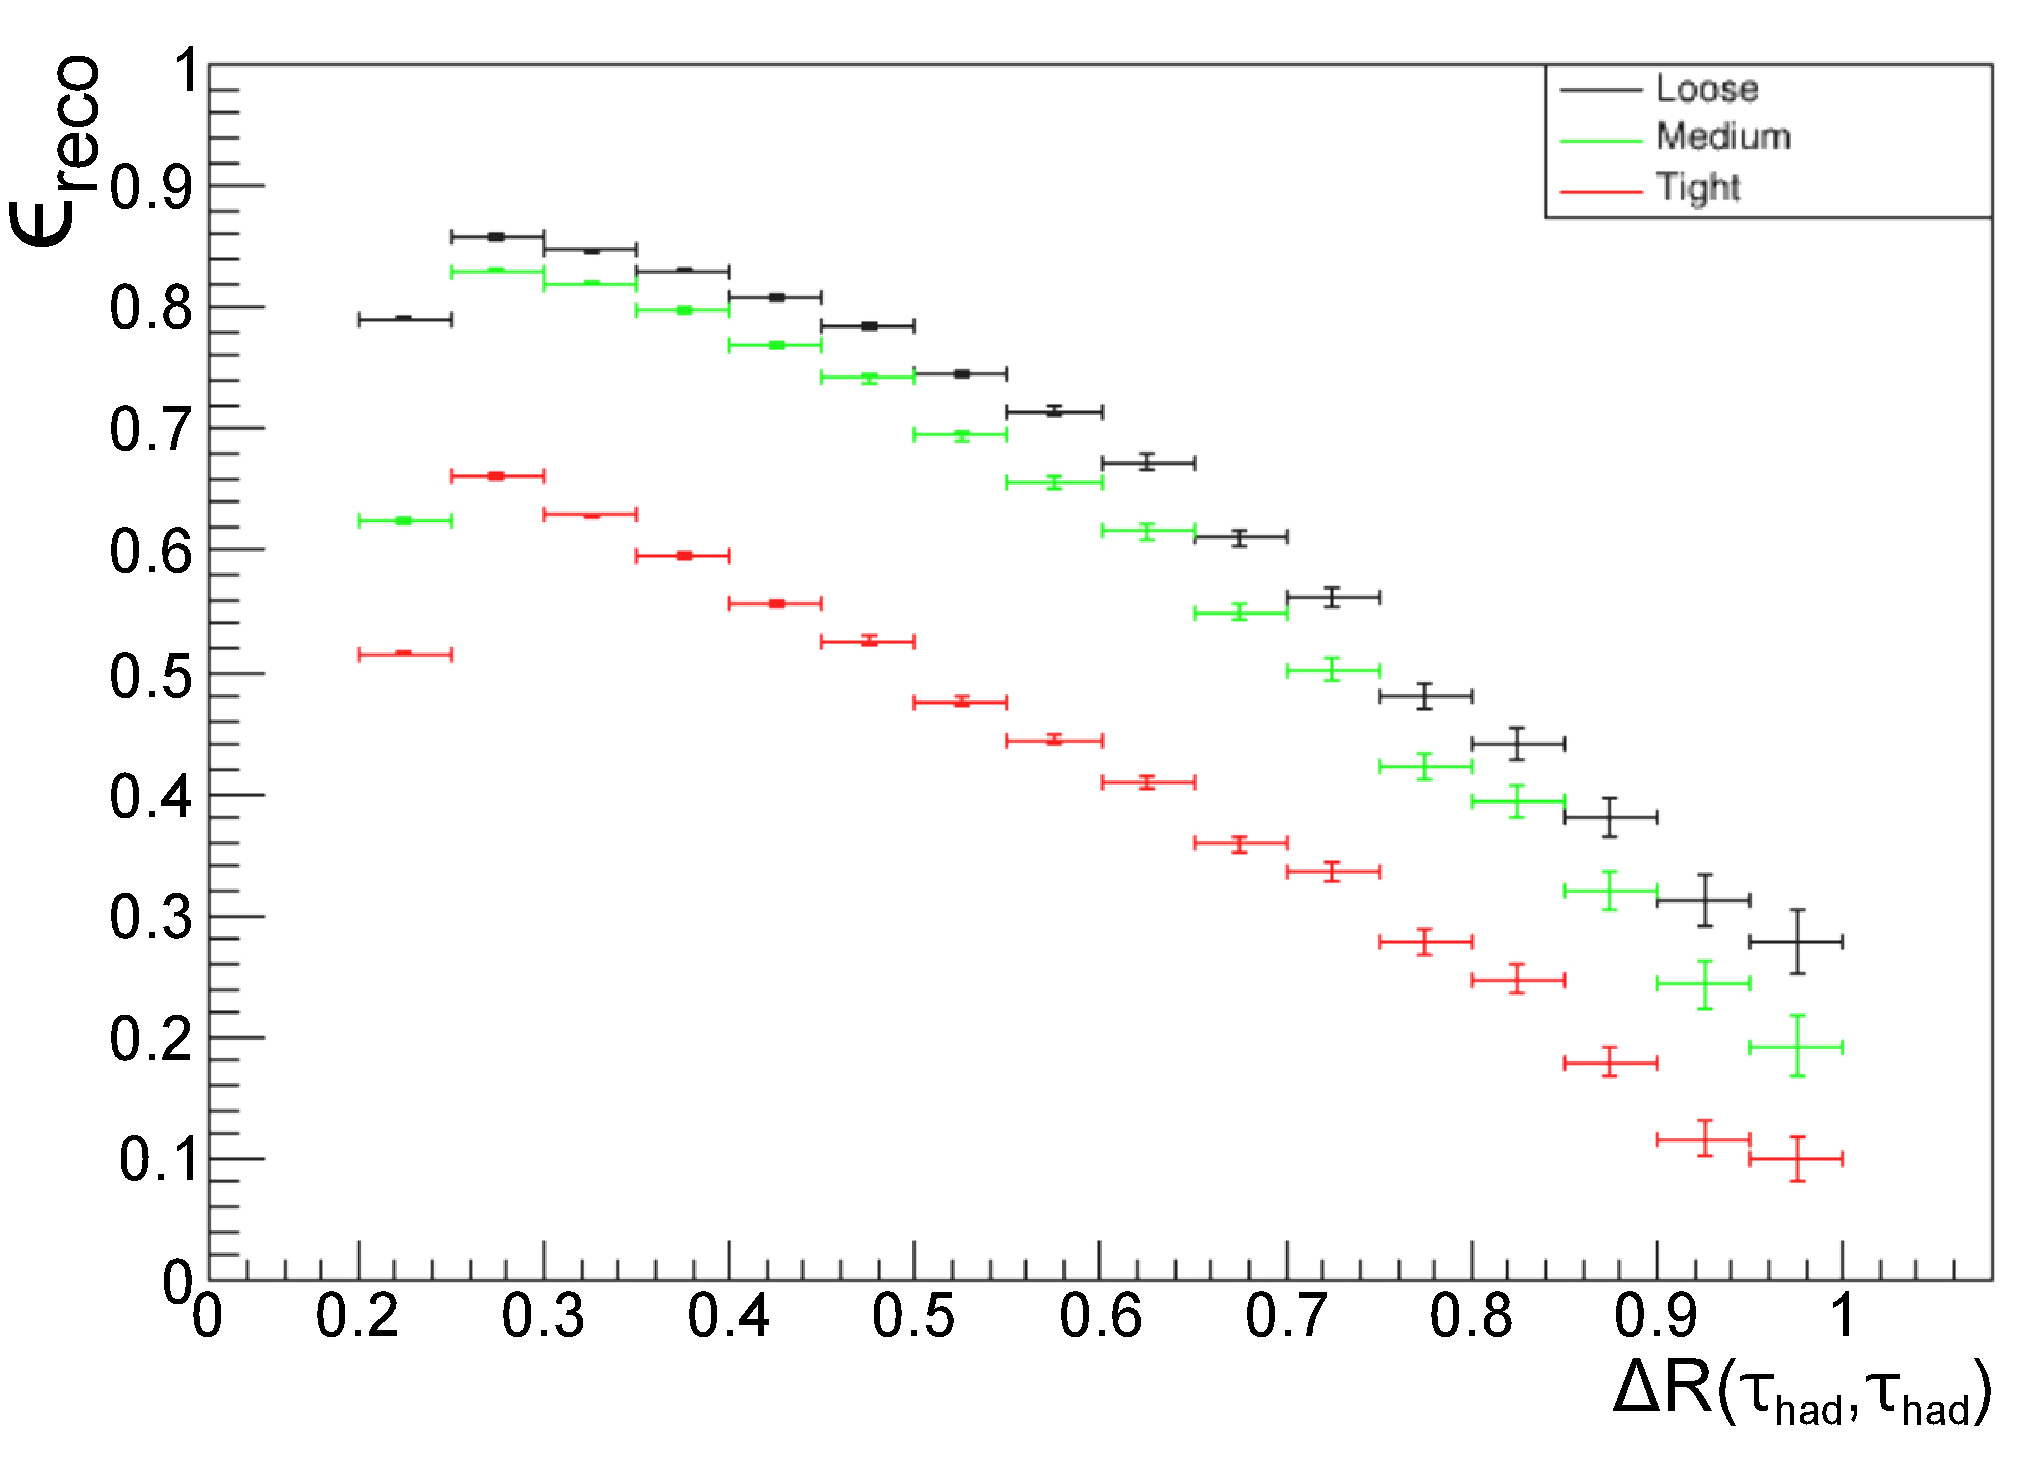
\includegraphics[width=0.99\marginparwidth]{Assets/Plots/DiTau/Reco/efficiency_dR.pdf}}
    \caption{Eficiencias de reconstrucción de objetos DiTau. Los colores representan distintos criterios de TM, donde los \textit{truth} \thads se encuentran: dentro del jet $R = 1$ del objeto (\textit{Loose}, en negro); a $\Delta R < 0.2$ de cualquier par de subjets (\textit{Medium}, en verde); a $\Delta R < 0.2$ de los subjets \textit{leading} y \textit{subleading} (\textit{Tight}, en rojo).}
    \label{fig:ch3:ditau:reco_efficiency}
\end{marginfigure}



\subsection{Identificación}

En el proceso de identificación se discrimina entre los objetos DiTau provenientes de 2 \thads físicos y los objetos DiTau \textit{fakes} (falsos), que por el contrario no están constituidos por \ttaus. Estos últimos pueden provenir de depósitos de energía reconstruidos en jets con topologías similares, provenientes de la interacción de otras partículas con los detectores, o de jets de \textit{pile-up}. Este proceso se realiza utilizando un \textit{Boosted Decision Tree} (BDT), una técnica de análisis multivariable compuesta de múltiples árboles de decisión interconectados, comunmente utilizada en física de altas energías para clasificar objetos y eventos~\citeonly{Coadou2013,pml1Book}.

\begin{marginfigure}
    \centering
    \definecolor{bkg_node}{cmyk}{0, 0.48, 0.25, 0}
\definecolor{sig_node}{cmyk}{0.16, 0.07, 0, 0}
\begin{tikzpicture}
    \tikzset{
        font=\sffamily,
        every node/.style = {
            draw=darkgray,
            thin,
            align=center,
            inner sep=0pt,
        },
        grad/.style = {
            shading=axis,
            top color=sig_node,
            bottom color=bkg_node,
        },
        arrow/.style = {
            -{latex[scale=0.7]},
            black,
            thick,
        },
        midbox/.style = {
            fill=white,
            draw=Burgundy,
            minimum height=4.1mm,
            inner sep=0.7mm,
            rectangle,
            rounded corners=2,
            font=\tiny,
        },
    }
    \node[fill=Goldenrod, circle, minimum size=7mm] (root) at (0,0) {Raíz};
    \node[below left=12mm and 11mm of root, shade, grad, circle, minimum size=7mm] (l1n1) {};
    \node[below right=12mm and 11mm of root, shade, grad, circle, minimum size=7mm] (l1n2) {};
    %
    \node[below left=12mm and 2mm of l1n1, fill=bkg_node, circle, minimum size=7mm] (l2n1) {B};
    \node[below right=12mm and 2mm of l1n1, fill=sig_node, circle, minimum size=7mm] (l2n2) {S};
    \node[below left=12mm and 2mm of l1n2, shade, grad, circle, minimum size=7mm] (l2n3) {};
    \node[below right=12mm and 2mm of l1n2, fill=sig_node, circle, minimum size=7mm] (l2n4) {S};
    %
    \node[below left=12mm and 2mm of l2n3, fill=bkg_node, circle, minimum size=7mm] (l3n1) {B};
    \node[below right=12mm and 2mm of l2n3, fill=sig_node, circle, minimum size=7mm] (l3n2) {S};
    %
    \draw[arrow] ([shift={(-1mm, 0.1mm)}]root.south) -- (l1n1.north) node[midbox, pos=0.45] {$x_i < c_1$};
    \draw[arrow] ([shift={(+1mm, 0.1mm)}]root.south) -- (l1n2.north) node[midbox, pos=0.45] {$x_i \geq c_1$};
    %
    \draw[arrow] ([shift={(-1mm, 0.1mm)}]l1n1.south) -- (l2n1.north);
    \node[midbox] at ($(l1n1)!0.45!(l2n1) + (-3mm, 0mm)$) {$x_j < c_2$};
    \draw[arrow] ([shift={(+1mm, 0.1mm)}]l1n1.south) -- (l2n2.north);
    \node[midbox] at ($(l1n1)!0.45!(l2n2) + (+3mm, 0mm)$) {$x_j \geq c_2$};
    \draw[arrow] ([shift={(-1mm, 0.1mm)}]l1n2.south) -- (l2n3.north);
    \node[midbox] at ($(l1n2)!0.45!(l2n3) + (-3mm, 0mm)$) {$x_j < c_3$};
    \draw[arrow] ([shift={(+1mm, 0.1mm)}]l1n2.south) -- (l2n4.north);
    \node[midbox] at ($(l1n2)!0.45!(l2n4) + (+3mm, 0mm)$) {$x_j \geq c_3$};
    %
    \draw[arrow] ([shift={(-1mm, 0.1mm)}]l2n3.south) -- (l3n1.north);
    \node[midbox] at ($(l2n3)!0.45!(l3n1) + (-3mm, 0mm)$) {$x_k < c_4$};
    \draw[arrow] ([shift={(+1mm, 0.1mm)}]l2n3.south) -- (l3n2.north);
    \node[midbox] at ($(l2n3)!0.45!(l3n2) + (+3mm, 0mm)$) {$x_k \geq c_4$};
\end{tikzpicture}

    \caption{Esquema genérico de un árbol de decisiones binarias. Los nodos finales (hojas) indican el resultado del proceso de clasificación, siendo en este caso ``S'' un objeto o evento identificado como señal y ``B'' un objeto o evento identificado como fondo.}
    \label{fig:ch3:ditau:bdt_schematic}
\end{marginfigure}

Cada árbol de decisión se encuentra compuesto por una secuencia consecutiva de nodos en los que se realizan decisiones binarias, generando \textit{ramificaciones} del nodo raíz original, como podemos observar en el diagrama de la \cref{fig:ch3:ditau:bdt_schematic}. Los cálculos en cada nodo utilizan como entradas los resultados de los nodos anteriores, produciendo un veredicto final binario al alcanzar un número máximo de nodos. En analogía al concepto de árbol, los nodos finales reciben el nombre de \textit{hojas}. El valor de los cortes realizados en cada nodo es optimizado mediante un entrenamiento supervisado, utilizando muestras ya clasificadas.

Si bien los árboles de decisión son rápidos de entrenar y fáciles de interpretar, el uso de un único árbol no presenta una buena capacidad discriminante. Por lo tanto, para mejorar el rendimiento del clasificador se suelen emplear múltiples árboles de decisión, realizando un voto de mayoría pesado entre sus resultados, donde los pesos son también obtenidos por medio del entrenamiento.

El entrenamiento de los BDTs comprende el uso de un algoritmo de ampliación (\textit{boosteo}\sidenote{Pese a la nomenclatura accidentada, no hace falta aclarar que nada tiene que ver este procedimiento con las transformaciones de Lorentz.}), en el que luego de entrenar el primer árbol, los árboles siguientes son utilizados para corregir los errores anteriores\sidenote{
Suponiendo que contamos con $N_{\text{tree}}$ árboles $T_k$ y un conjunto $D_1$ de datos para el entrenamiento. Sea una función sobre los datos
\[ 
    \mathcal{I}_k(i) = 
    \begin{cases}
        1, & \text{$i$ bien clasificado en $T_k$,}\\
        0, & \text{c.c.}
    \end{cases}
\]
Definimos la fracción de clasificación errónea
\[ \varepsilon_k = \frac{\sum_i w_i^k \mathcal{I}_k(i)}{\sum_i w_i^k}, \]
donde $w_i^k$ es un peso asignado a cada dato $i$ en $D_k$, con $w_i^1 = 1$. El procedimiento de \textit{boosteo} será:
\begin{algorithmic}[1]
\For{$k$ in $1$..$N_{\text{tree}}$}
    \State Entrenar árbol $T_k$ con los datos $D_k$
    \State $\alpha_k \gets \beta \log(\frac{1 - \varepsilon_k}{\varepsilon_k})$
    \State $w_i^{k+1} \gets w_i^k e^{\alpha_k \mathcal{I}_k(i)}$
\EndFor
\end{algorithmic}
con $\beta$ un parámetro característico del BDT.
}. El resultado del BDT para cada conjunto de variables $\vb{x}$ será entonces
\[ T(\vb{x}) = \inv{\sum_k \alpha_k} \sum_{k = 1}^{N_{\text{tree}}} \alpha_k T_k(\vb{x}), \]
adquiriendo valores en el rango $-1 \leq T \leq +1$, donde $\alpha_k$ es un peso asignado al resultado de cada árbol $T_k$.

La selección del conjunto de variables a ingresar en el BDT contempla minimizar las diferencias en la eficiencia de identificación entre las muestras de \SI{20}{\GeV} y \SI{60}{\GeV} utilizadas para el entrenamiento. Muchas de estas variables son análogas a las utilizadas en el proceso de identificación de los $\tau_{\text{had}}$ individuales, aquí aplicadas a los subjets \textit{leading} y \textit{subleading} (LyS). A continuación serán enumeradas y definidas:
\begin{itemize}
    \item $n_{\text{isotracks}}$: Número de trazas en la zona de aislamiento del objeto DiTau.

    \item $\displaystyle f^{\text{(sub)lead}}_{\text{track}} = \frac{p_T^{\text{lead trk}}}{p_T^{\text{subjet}}}$: Fracción de energía del \textit{track} principal en los subjets LyS.
    \item $\displaystyle f^{\text{(sub)lead}}_{\text{subjet}} = \frac{p_T^{\text{(sub)lead}}}{p_T^{\text{seed}}}$: Fracción de energía de los subjets LyS respecto al jet $R = 1$ que los incluye.
    \item $\log(m_{\text{tracks}}^{\text{(sub)lead}})$: masa del sistema compuesto por las trazas de los subjets LyS.
    
    \item $\log\abs{d_{\text{0,lead-track}}^{\text(sub)lead}}$: Parámetro de impacto de la traza de mayor energía en los subjets LyS.
    \item $R^{\text{(sub)lead}}_{\text{max}}$: Radio máximo de la reconstrucción de los subjets LyS.
    \item $\displaystyle R^{\text{(sub)lead}}_{\text{core}} = \frac{\sum_i^{\Delta R_i < 0.1} p_{T, i}^{\text{trk}} \Delta R_i}{\sum_i^{\Delta R_i < 0.1} p_{T, i}^{\text{trk}}}$: Promedio de las distancias angulares de las trazas en la zona \text{core} ($\Delta R < 0.1$) de los subjets LyS, pesados por su momento transverso.
    \item $\displaystyle R_{\text{track}} = \frac{\sum_{\text{(sub)lead}} \sum_i^{\Delta R_i < 0.2} p_{T, i}^{\text{trk}} \Delta R_i}{\sum_{\text{(sub)lead}} \sum_i^{\Delta R_i < 0.2} p_{T, i}^{\text{trk}}}$: Promedio de las distancias angulares de las trazas en ambos subjets (LyS), pesados por su momento transverso.
    \item $\displaystyle R_{\text{isotrack}} = \frac{\sum_{\text{(sub)lead}} \sum_i^{\Delta R_i < 0.4} p_{T, i}^{\text{isotrk}} \Delta R_i}{\sum_{\text{(sub)lead}} \sum_i^{\Delta R_i < 0.4} p_{T, i}^{\text{isotrk}}}$: Promedio de las distancias angulares de las trazas en la zona de aislamiento ($0.2 < \Delta R < 0.4$) de ambos subjets (LyS), pesados por su momento transverso.
    \item $\Delta R(\tau_1, \tau_2)$: Distancia angular entre los subjets LyS.
\end{itemize}
Las distribuciones para señal (muestra $t\bar{t}(X \to \tau_{\text{had}} \tau_{\text{had}})$, con $m_X = \SI{20}{\GeV}$) y fondo ($t\bar{t}$ con filtro solo-hadrónico) de las variables utilizadas se exhiben en la \cref{fig:ch3:ditau:bdt_vars}.

\begin{marginfigure}[-18em]
    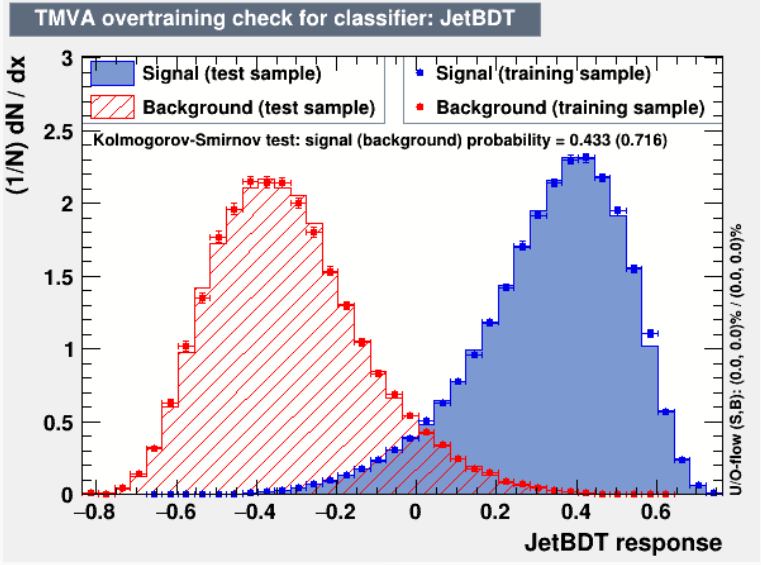
\includegraphics[width=0.99\linewidth]{Assets/Plots/DiTau/ID/TMVA.png}
    \caption{Distribuciones de puntaje del BDT luego del entrenamiento, utilizando eventos $t\bar{t}$ \textit{all-hadronic} como fondo y eventos \textit{truth-matched} $t\bar{t}(X \to \tau\tau)$ con $m_X = \SI{20}{\GeV}$ como señal. Solo se aplicó un requerimiento en el número de \textit{tracks} dentro de los subjets LyS y un corte en $p_T > \SI{20}{\GeV}$ en todos los objetos.}
    \label{fig:ch3:ditau:bdt_output}
\end{marginfigure}

En el procedimiento de identificación de los objetos DiTau se emplea un BDT de 1500 árboles, con una profundidad máxima de 3 niveles en cada árbol y parámetro de boosteo $\beta = 0.2$. EL BDT fue entrenado con el framework TMVA~\cite{hoecker2009tmva} provisto por ROOT, utilizando el algoritmo \texttt{AdaBoost}. Se utilizaron $10^6$ eventos de señal del proceso $t\bar{t}(X\to\tau\tau)$ con masas de \num{20} y \SI{60}{\GeV} (DSIDs \texttt{425500} y \texttt{425501}), seleccionando solo eventos con DiTaus decayendo hadrónicamente. Como fondo se utilizaron $10^6$ eventos de una muestra de $t\bar{t}$ \textit{all-hadronic} (donde a los $W^\pm$ del decaimiento de los quarks $t$ solo se les permitide decaer hadrónicamente), para mejorar el rendimiento de identificación contra jets (que, como se verá más adelante, son la contribución dominante a los fondos). Todos los DiTau considerados en el entrenamiento debieron tener subjets LyS con 1 o 3 \textit{tracks} y satisfacer los cortes $p_T > \SI{20}{\GeV}$ y $\Delta R_{\text{truth}} < 1.0$, donde $\Delta R_{\text{truth}}$ es la separación angular del par de \ttaus indicada por el generador (antes del proceso de simulación del detector y posterior reconstrucción).

\begin{marginfigure}[-7em]
    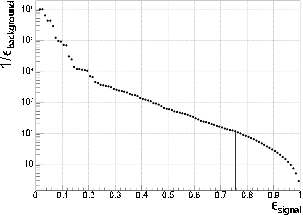
\includegraphics[width=0.99\linewidth]{Assets/Plots/DiTau/ID/efficiency_sig-vs-bkg_60GeV.pdf}
    \caption{Distribuciones de eficiencia de identificación para señal ($t\bar{t}(X \to \tau\tau)$, con $m_X = \SI{60}{\GeV}$) y fondo ($t\bar{t}$ \textit{all-hadronic}).}
    \label{fig:ch3:ditau:id_efficiency}
\end{marginfigure}

La \cref{fig:ch3:ditau:bdt_output} exhibe las distribuciones del puntaje del BDT luego del entrenamiento, para una muestra TM de señal de \SI{20}{\GeV}. Considerando un criterio de rechazo de fondo de 1\% (solo permitiendo que el 1\% de los eventos de fondo iniciales sean mal-identificados), el algoritmo de identificación resulta con una eficiencia media de señal de 75\%, correspondiente a un corte en el puntaje del BDT para los eventos de señal de $BDT > 0.22$. En particular, la eficiencia resulta de 73\% en eventos de la muestra de \SI{20}{\GeV} y 77\% en la muestra de \SI{60}{\GeV} (\cref{fig:ch3:ditau:id_efficiency}). La elección de variables realizada resulta en un rendimiento estable ante la masa invariante del objeto DiTau, como podemos observar en la \cref{fig:ch3:ditau:bdt_vs_m}.

\begin{marginfigure}[-2em]
    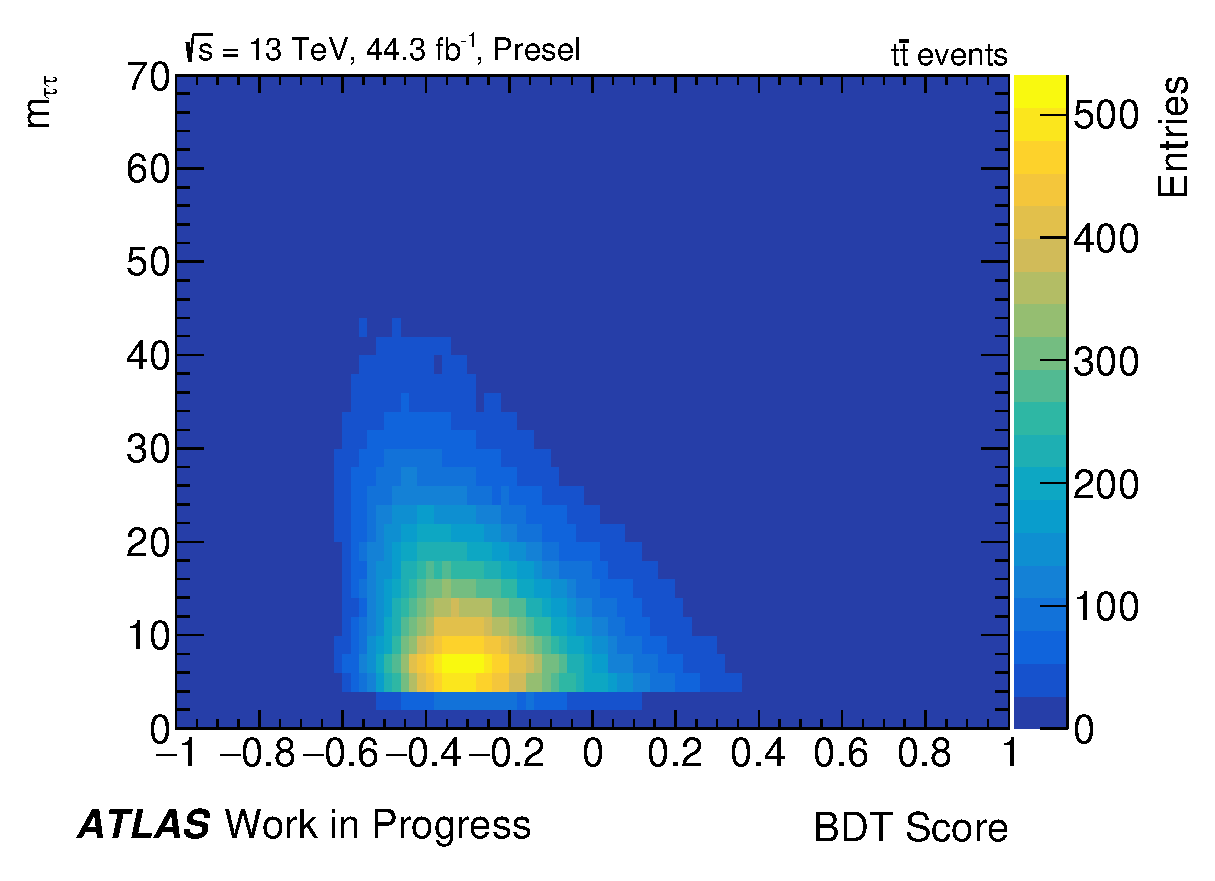
\includegraphics[width=0.99\linewidth]{Assets/Plots/DiTau/Presel/ttbar_leptonOR/h_mc16d_ttbar_ditau_bdt_m.eps}
    \caption{Distribuciones de $BDT$ vs $m$ de los objetos DiTau \textit{fake} provenientes de jets mal-identificados, en la muestra de $t\bar{t}$.}
    \label{fig:ch3:ditau:bdt_vs_m}
\end{marginfigure}

Combinando todos los resultados de eficiencia, se estableció el rango de masas de la presente búsqueda en $\SI{20}{\GeV} \leq m_X \leq \SI{60}{\GeV}$. El límite superior corresponde a la transición del régimen \textit{boosted} al régimen \textit{resolved} en los eventos de señal, siendo en la mayoría de los casos la separación de \ttaus de mayor masa $\Delta R \gtrsim 1.0$, superior al límite de reconstrucción de los objetos DiTau. El límite inferior se encuentra determinado por las distribuciones de $p_T$ de los \ttaus: para masas $m_X \lesssim \SI{20}{\GeV}$, los leptones serán producidos con muy poco momento transverso (\textit{soft taus}), perdiéndose su estructura característica, utilizada en la identificación.

\clearpage{}
\begin{figure*}[th!]
    \centering
    \setlength{\individualPlotWidth}{0.3\textwidth}
    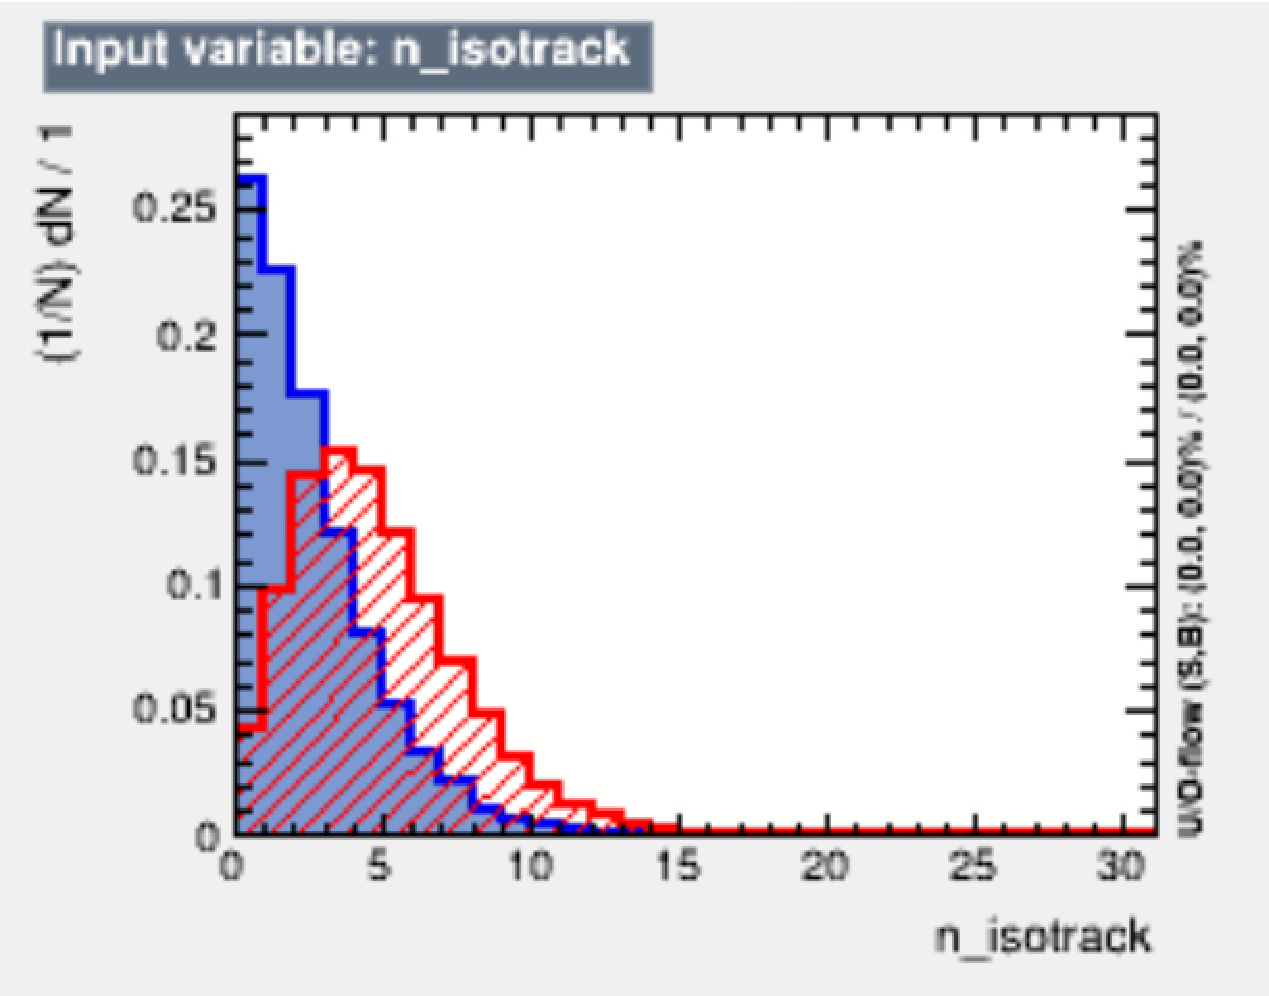
\includegraphics[width=\individualPlotWidth]{Assets/Plots/DiTau/BDT_vars/n_isotracks.pdf}
    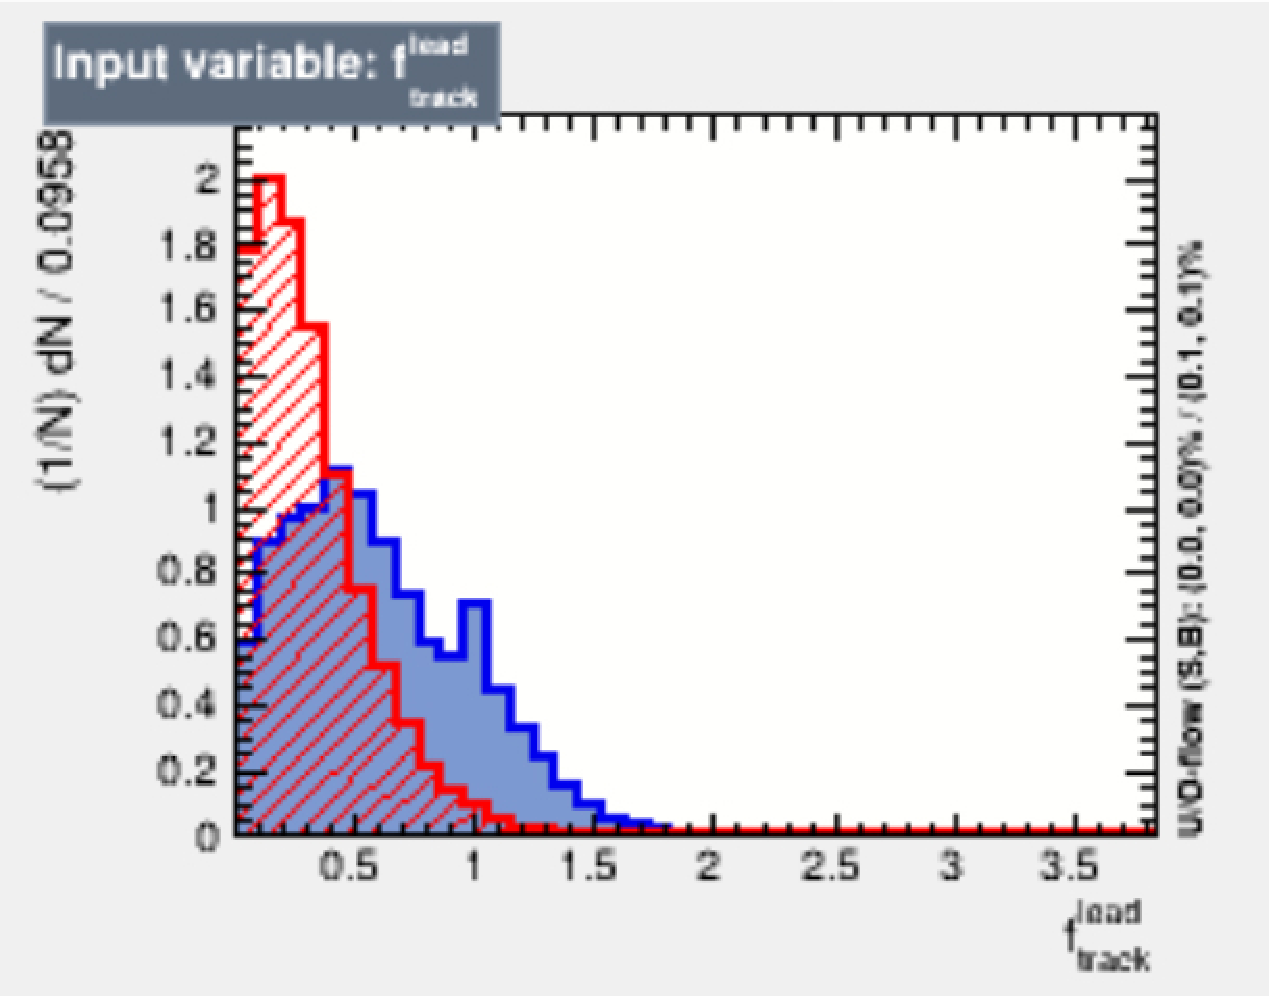
\includegraphics[width=\individualPlotWidth]{Assets/Plots/DiTau/BDT_vars/f_lead_track.pdf}
    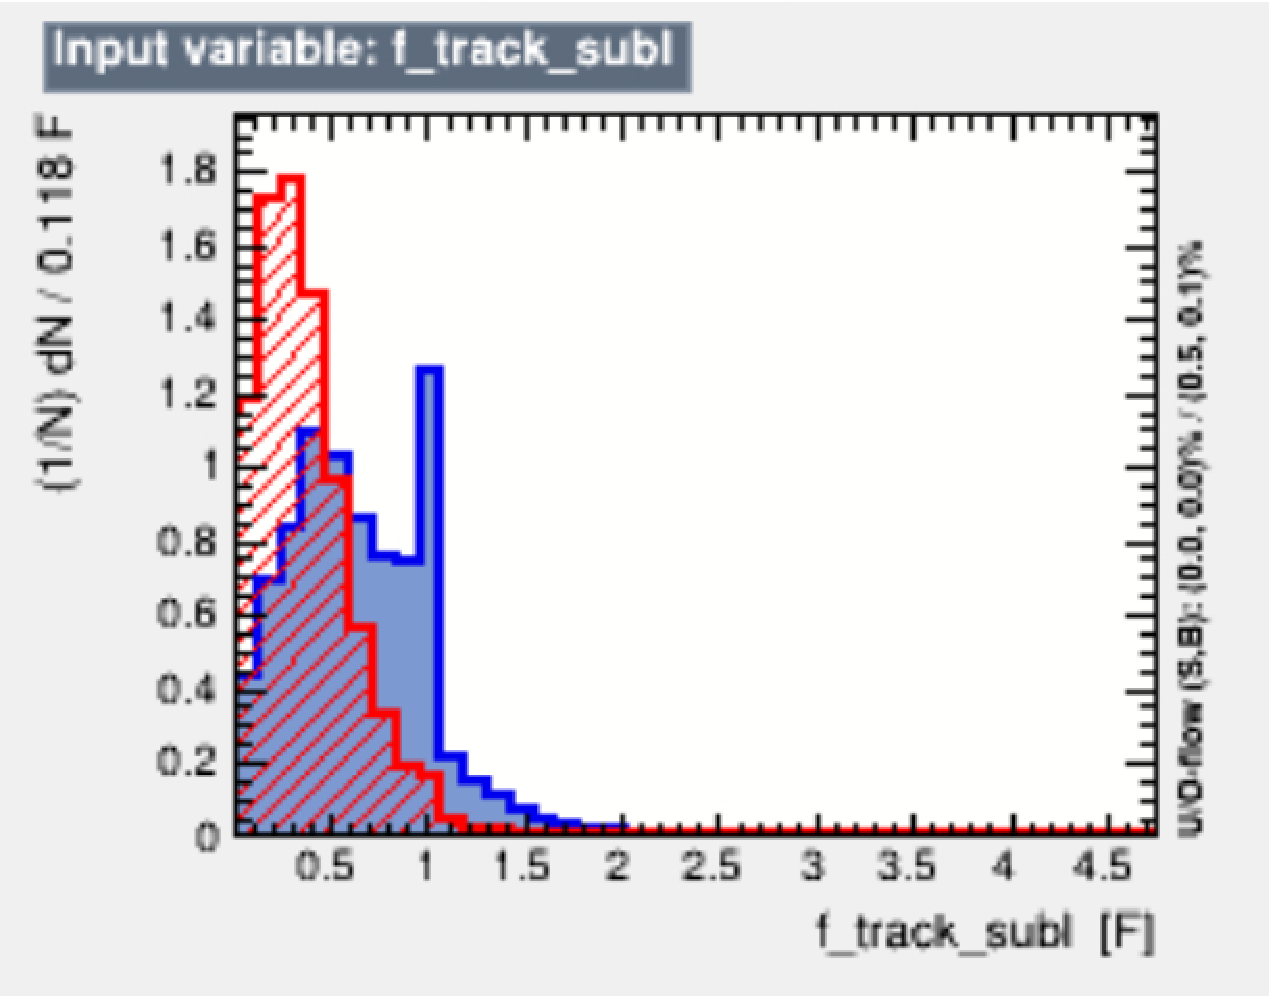
\includegraphics[width=\individualPlotWidth]{Assets/Plots/DiTau/BDT_vars/f_subl_track.pdf}
    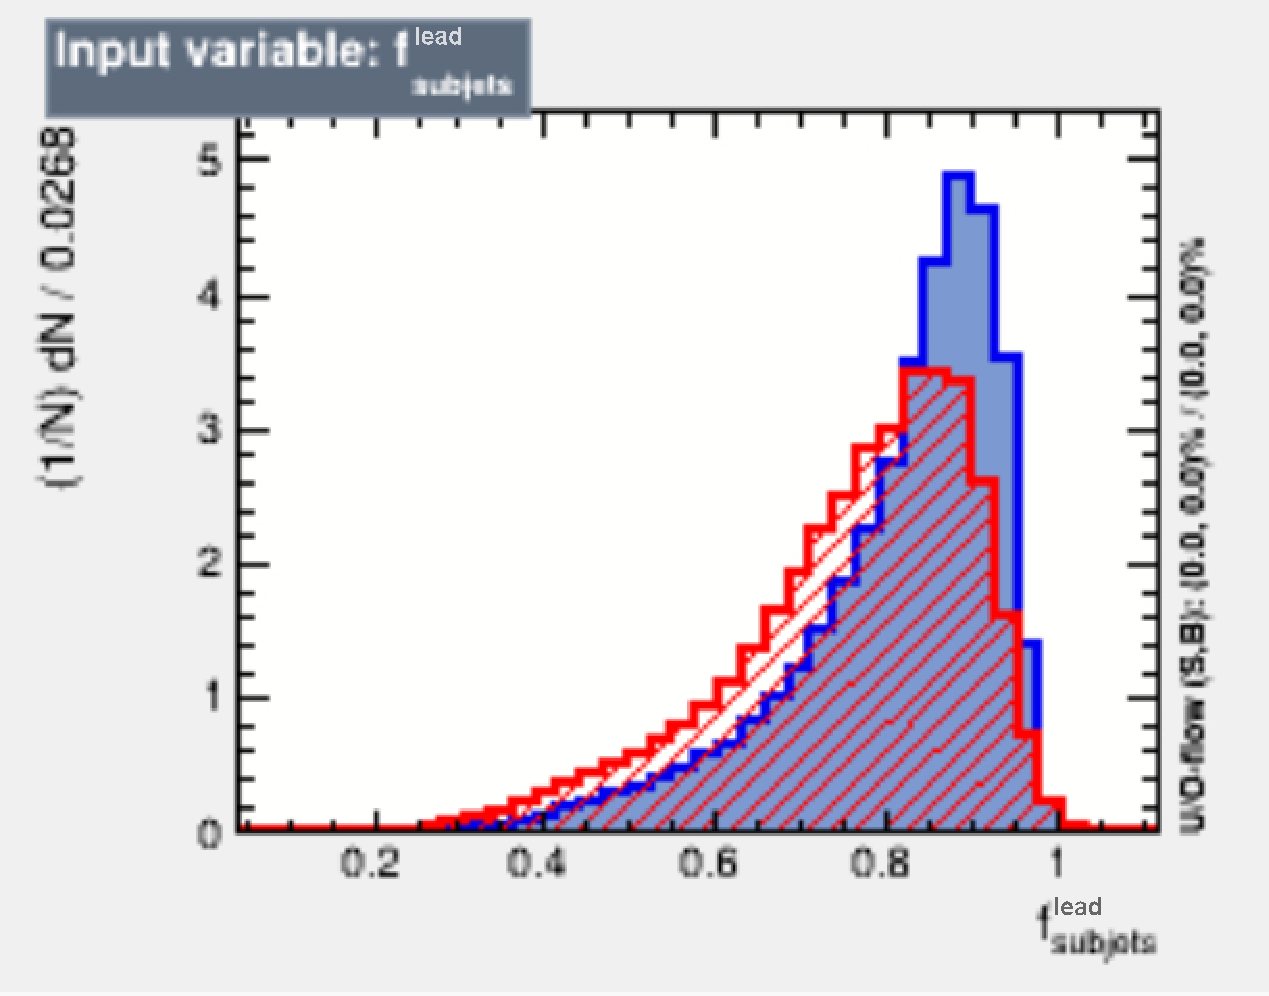
\includegraphics[width=\individualPlotWidth]{Assets/Plots/DiTau/BDT_vars/f_subjet_lead.pdf}
    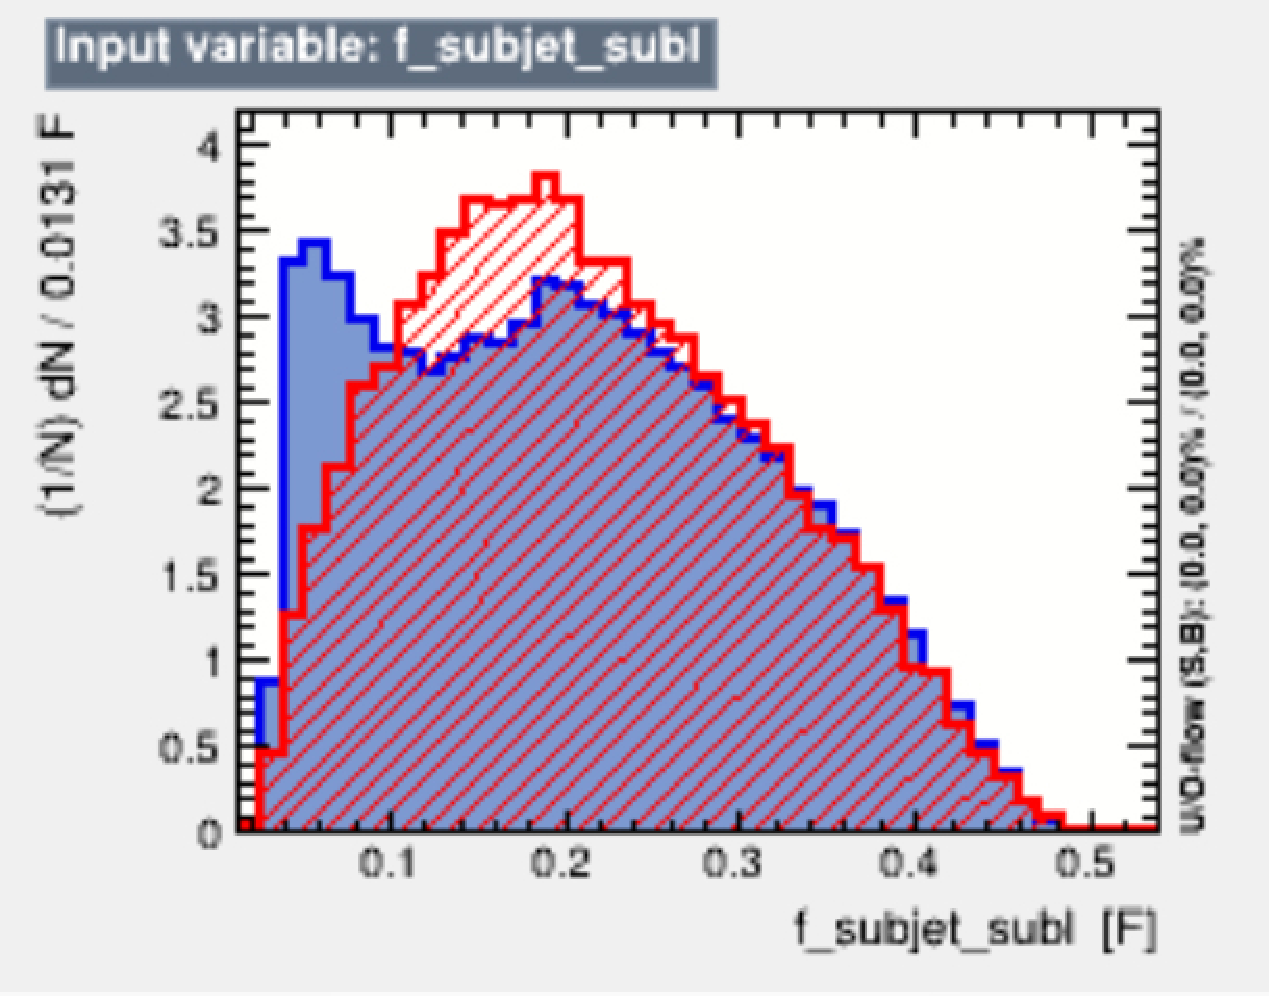
\includegraphics[width=\individualPlotWidth]{Assets/Plots/DiTau/BDT_vars/f_subjet_subl.pdf}
    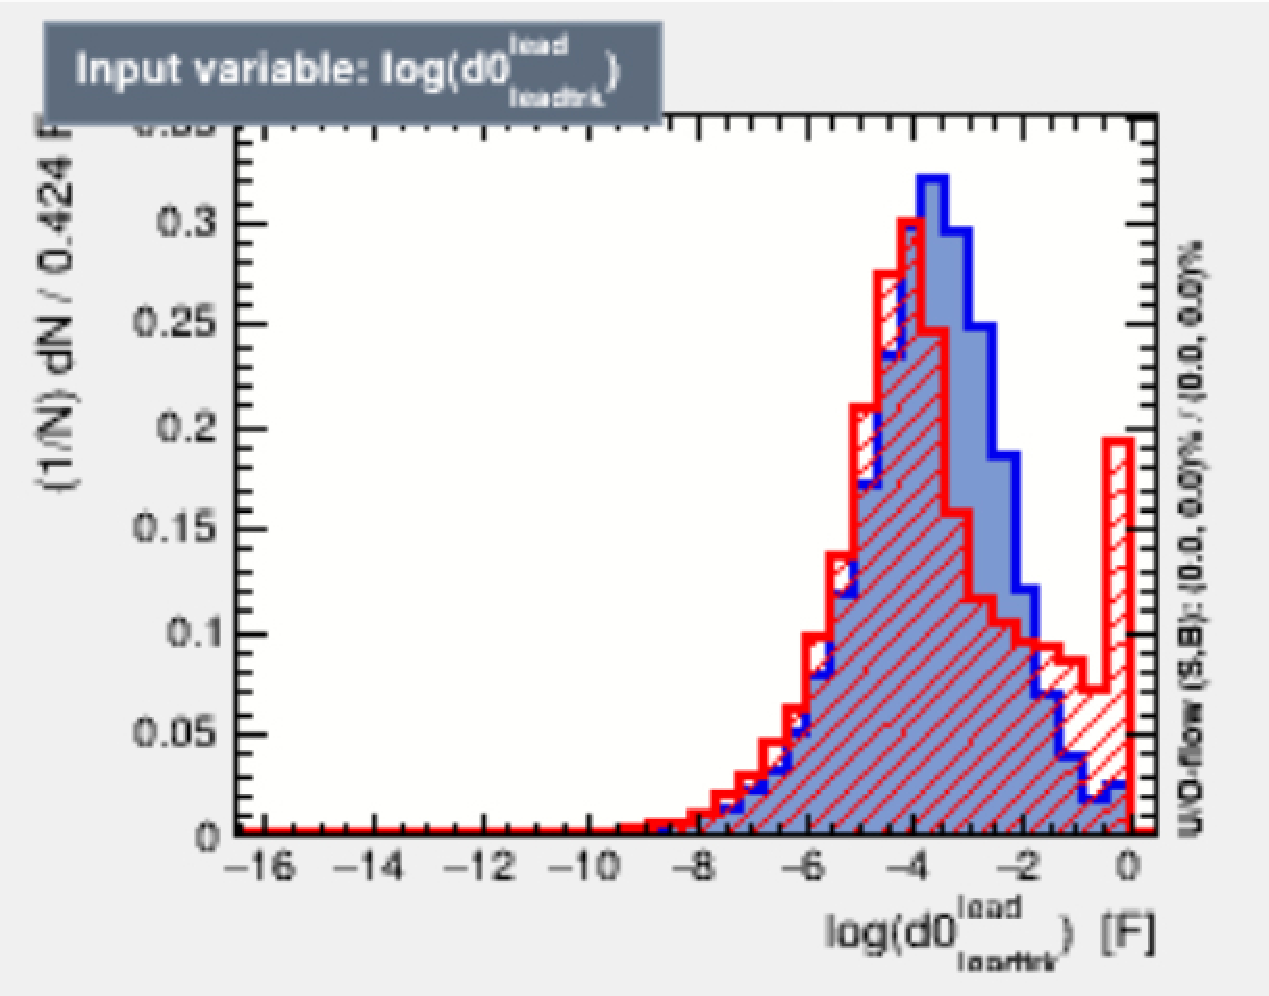
\includegraphics[width=\individualPlotWidth]{Assets/Plots/DiTau/BDT_vars/d0_leadtrack_lead.pdf}
    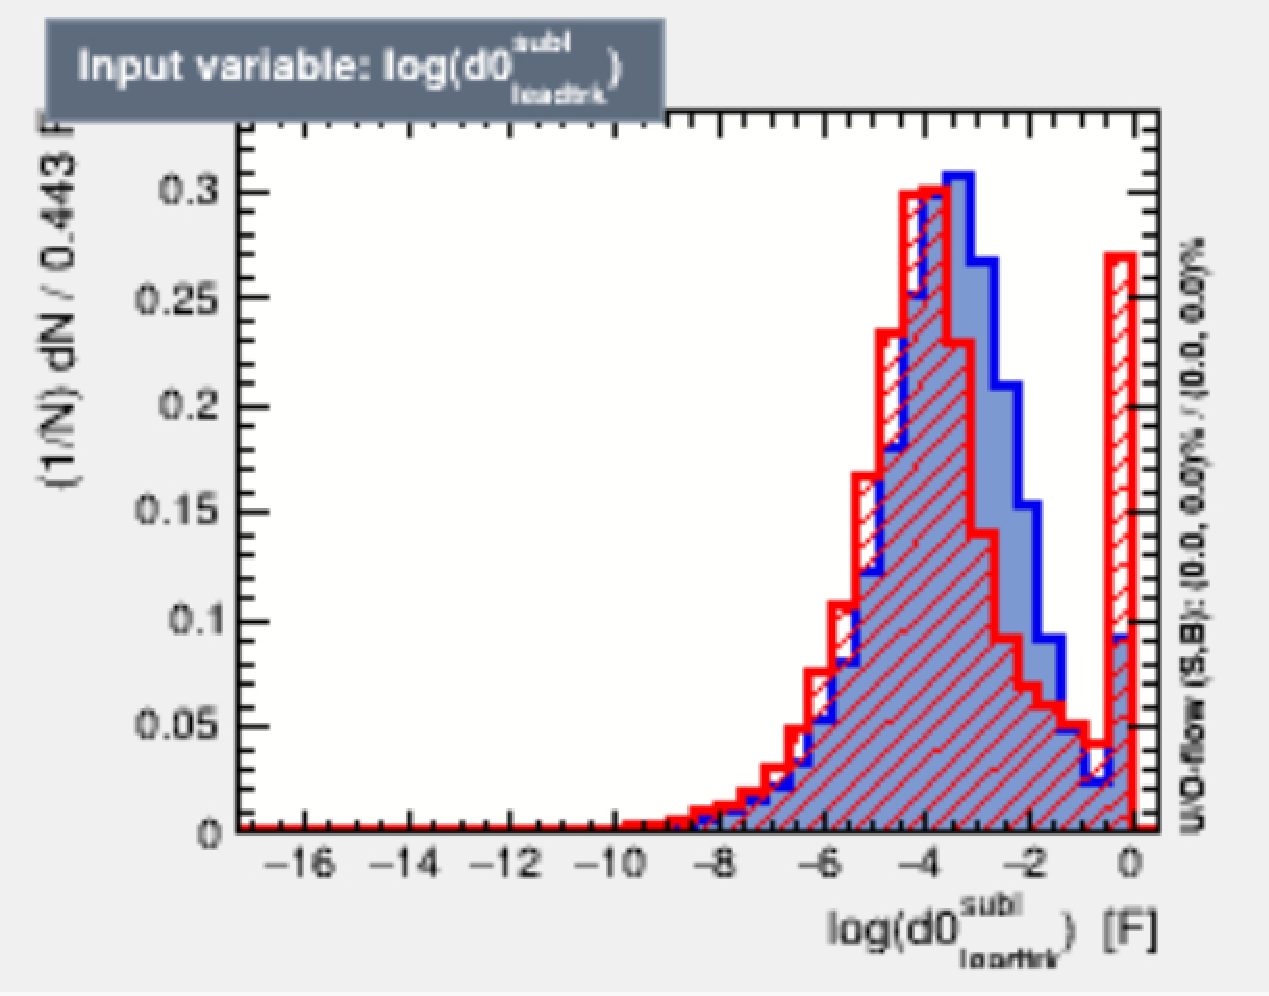
\includegraphics[width=\individualPlotWidth]{Assets/Plots/DiTau/BDT_vars/d0_leadtrack_subl.pdf}
    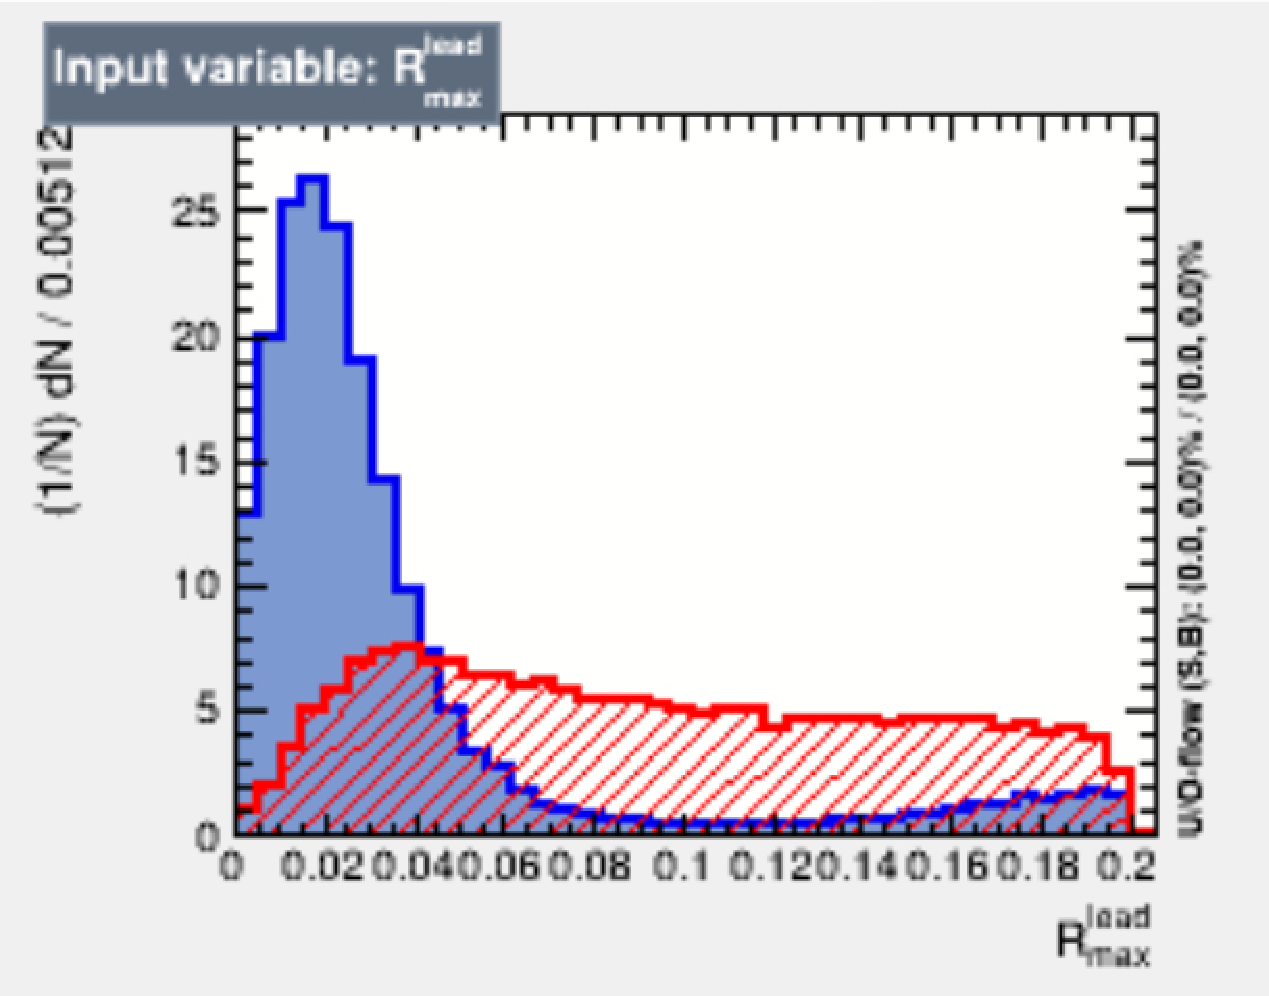
\includegraphics[width=\individualPlotWidth]{Assets/Plots/DiTau/BDT_vars/R_lead_max.pdf}
    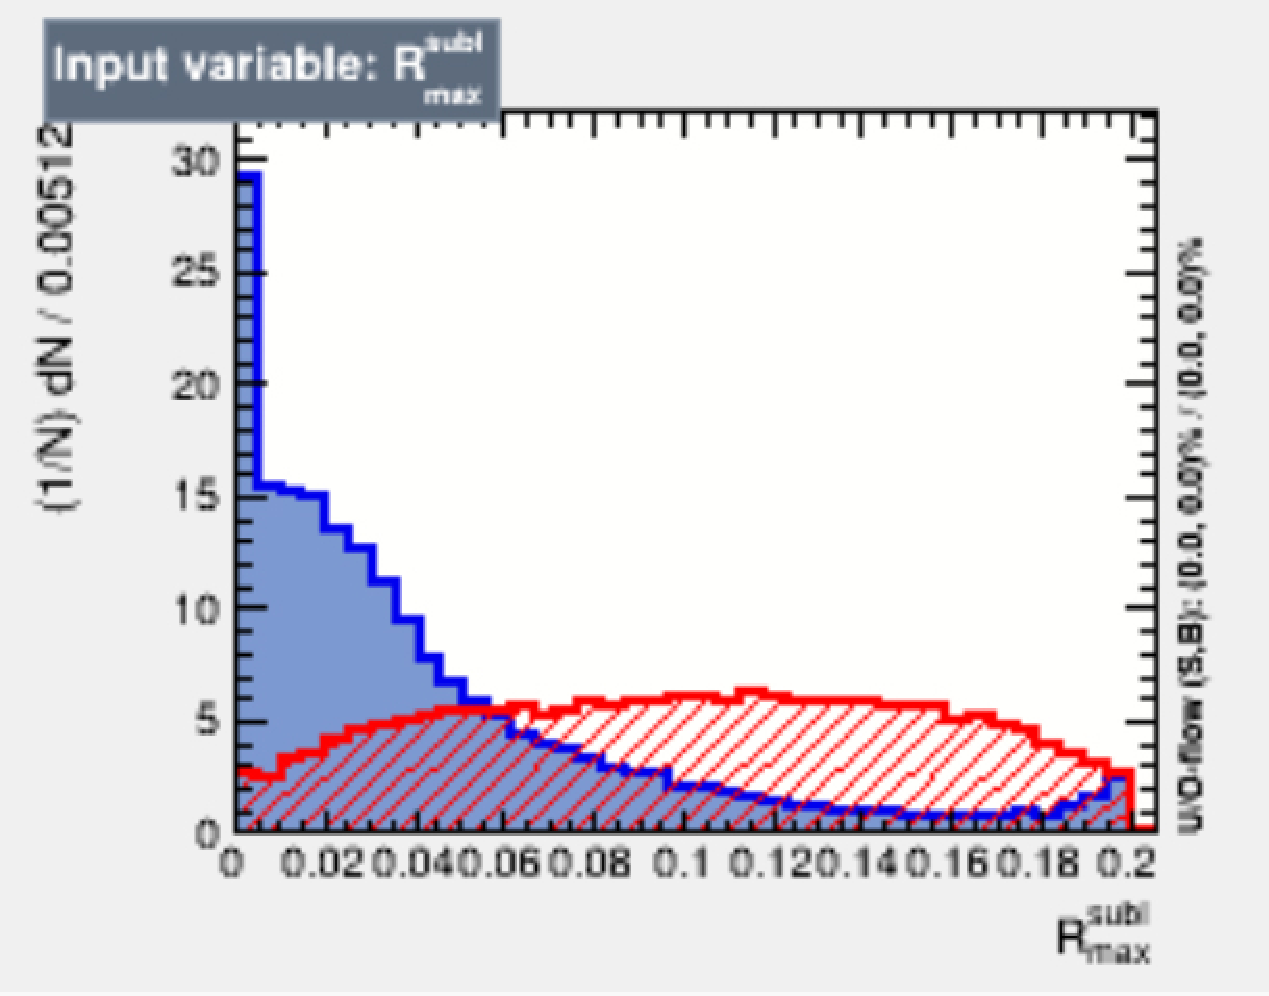
\includegraphics[width=\individualPlotWidth]{Assets/Plots/DiTau/BDT_vars/R_subl_max.pdf}
    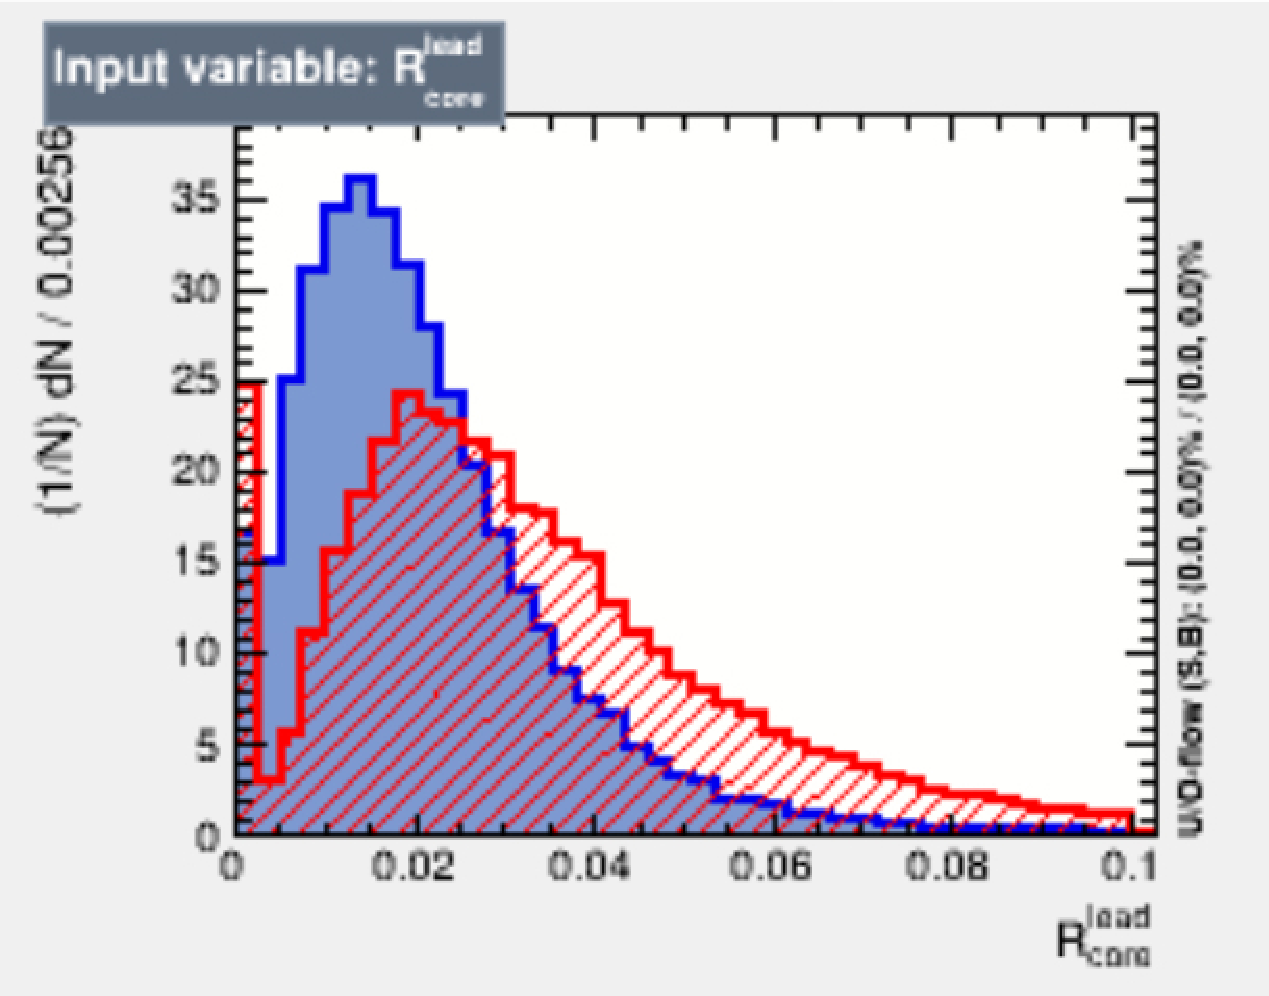
\includegraphics[width=\individualPlotWidth]{Assets/Plots/DiTau/BDT_vars/R_lead_core.pdf}
    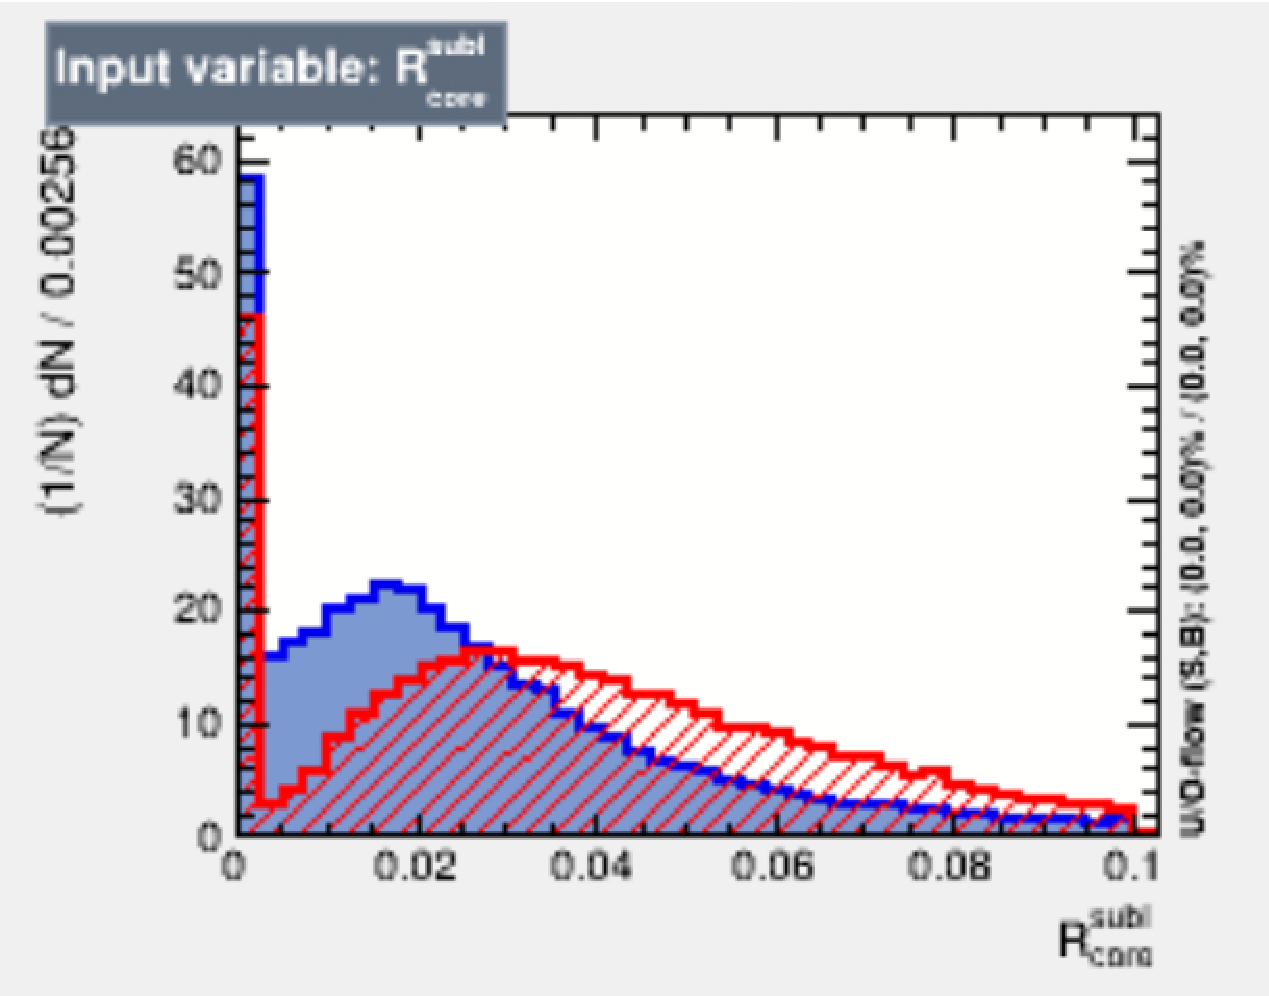
\includegraphics[width=\individualPlotWidth]{Assets/Plots/DiTau/BDT_vars/R_subl_core.pdf}
    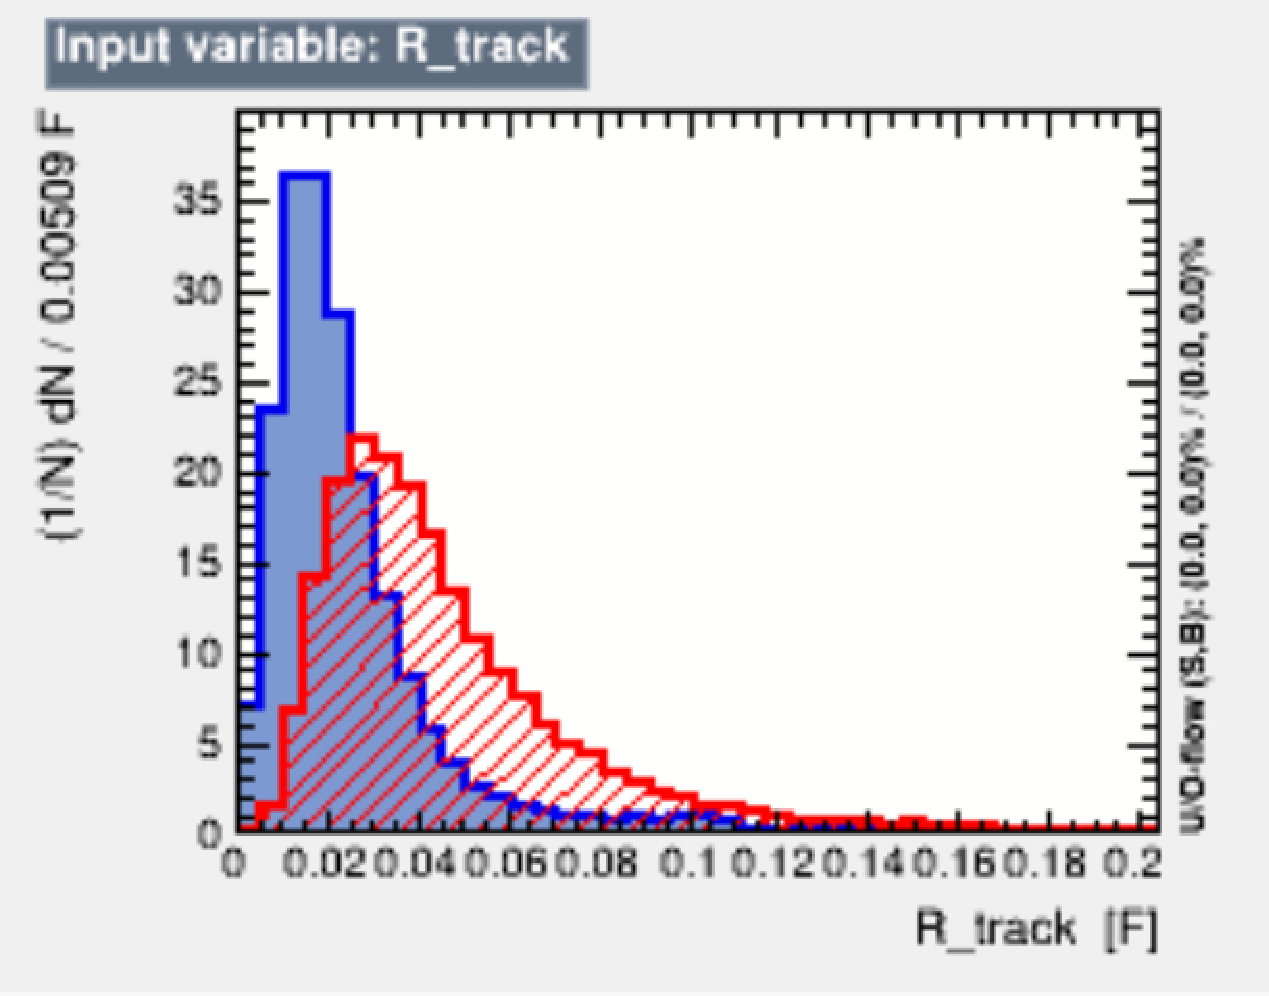
\includegraphics[width=\individualPlotWidth]{Assets/Plots/DiTau/BDT_vars/R_track.pdf}
    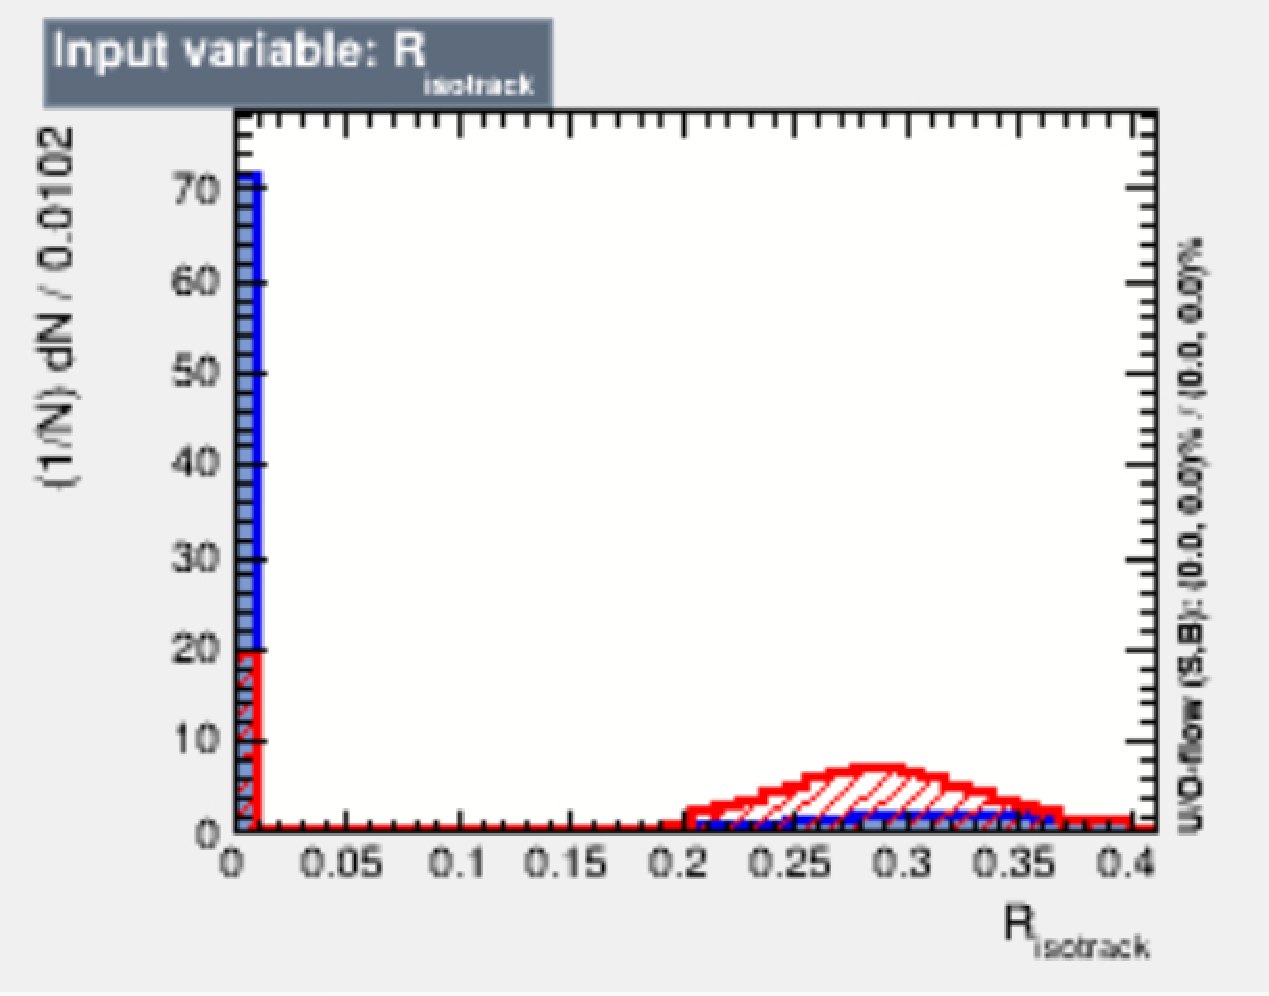
\includegraphics[width=\individualPlotWidth]{Assets/Plots/DiTau/BDT_vars/R_isotrack.pdf}\\

    \vspace{1em}
    \fullwidthCaption{Distribuciones de señal (\SI{20}{\GeV}, en azul) y fondo ($t\bar{t}$, en rojo) de las variables utilizadas en el BDT de identificación de los objetos DiTau.}
    \label{fig:ch3:ditau:bdt_vars}
\end{figure*}

\cleardoublepage{}